\documentclass[11pt,a4paper,fleqn]{article}
\usepackage{times}
\thispagestyle{empty}



\usepackage[T1]{fontenc}   % Silbentrennung

\usepackage[utf8x]{inputenc}
                                                                                                                             
\hyphenation{Acad-e-my}

\usepackage[bookmarks=true,bookmarksopen=true,%
breaklinks=true,%
draft=false,plainpages=false,hyperfootnotes=false,%
pdfauthor={Stefan Müller (Editor)},%
pdftitle={Proceedings of the 22nd International Conference on Head-Driven Phrase Structure Grammar},%
pdfkeywords={HPSG}%,
pdftex=true%
%ps2pdf=true  %ohne diesen Treiber geht der Zeilenumbruch in URLs
]{hyperref}% for pdf files
\hypersetup{colorlinks=false, pdfborder={0 0 0}}

\usepackage{pdfpages}
\pdfinclusioncopyfonts=1

\newcommand\formatauthor[2]{\begin{tabular}[t]{@{}c@{}}
  {\LARGE#1\strut}\\
  {\small#2\strut}\\
  \rule{\dimexpr0.5\linewidth-1em}{0pt}
  \end{tabular}\xhfill\ignorespaces}
\newcommand\xhfill{\hspace{1em plus 1fill}}

\begin{document}

\begin{center}
{\Large
                {\bfseries Proceedings of the 22nd International Conference on\par Head-Driven Phrase Structure Grammar\par}

                \vspace{8ex}

                     Nanyang Technological University (NTU), Singapore\\[\baselineskip]

                        Stefan M{\"u}ller (Editor)\\[\baselineskip]

                                2015\\[\baselineskip]

                          CSLI Publications\\[\baselineskip]

              http://csli-publications.stanford.edu/HPSG/2015 \\[4\baselineskip]

The papers are published under a \href{http://creativecommons.org/licenses/by/4.0/}{CC-BY license}:\\[3pt]
\href{http://creativecommons.org/licenses/by/4.0/}{http://creativecommons.org/licenses/by/4.0/}
}
\end{center}
\newpage
\tableofcontents

\newpage

\section{Editor's Note}
%% -*- coding:utf-8 -*-
The 22th International Conference on Head-Driven Phrase Structure Grammar (2015) was held at the Nanyang Technological University (NTU), Singapore.

The conference featured 3 invited talks, 15 papers, and 4 posters selected by the program committee 
(Anne Abeillé,
    Farrell Ackerman,
    Doug Arnold,
    Emily M. Bender (chair),
    Francis Bond,
    Gosse Bouma,
    George Broadwell,
    Rui Chaves,
    Philippa Cook,
    Ann Copestake,
    Kordula De Kuthy,
    Elisabet Engdahl,
    Dan Flickinger,
    Antske Fokkens,
    Danièle Godard,
    Petter Haugereid,
    Fabiola Henri,
    Anke Holler,
    Jong-Bok Kim,
    Jean-Pierre Koenig,
    Anna Kupsc,
    Bob Levine,
    Janna Lipenkova,
    Rob Malouf,
    Nurit Melnik,
    Philip Miller,
    Tsuneko Nakazawa,
    Joanna Nykiel,
    Gerald Penn,
    Adam Przepiorkowski,
    Frank Richter,
    Louisa Sadler,
    Pollet Samvellian,
    Sanghoun Song,
    Jesse Tseng,
    Steve Wechsler,
    Shûichi Yatabe and
    Eun-Jung Yoo).

A workshop on \emph{Verb Classes and the Scale of Change in Affected Arguments}
was attached to the conference. The workshop had six invited speakers and 
five regular papers. The workshop program was put together by František Kratochvíl and Joanna Ut-Seong Sio.

% wie viele?
%In total there were x  submissions to the conference and x submissions to the workshop.
We want to thank the respective program committees for putting this nice program together.

Thanks go to Francis Bond, who was
in charge of local arrangements, and his assistants Sanghoun Song, Michael Goodman,  Luis Morgado da Costa.
 

As in the past years the contributions to the conference proceedings are based on the five page abstract
that was reviewed by the respective program committees, but there is no additional reviewing of the
longer contribution to the proceedings.
To ensure easy access and fast publication we have chosen an electronic format.

The proceedings include all the papers except the one by Sanghoun Song, Chen Bo, Joanna Sio Ut
Seong, and Francis Bond titled \emph{An HPSG-based Analysis of Resultative Compounds in Chinese},
the one by Frank van Eynde, which is published in his book on predication, and the ones by I Wayan
Arka, Kazuko Yatsuhiro, Juwon Lee, and Hans
Uszkoreit. Most of the workshop contributions will be published in a separate volume and therefore
are also not included.





\newpage
\part{Contributions to the Main Conference}
\thispagestyle{empty}
\newpage
        \setcounter{page}{6}
        \phantomsection
        \addcontentsline{toc}{section}{Issa S. AlQurashi: An Analysis of Simple and Construct-State Noun Phrases in Modern Standard Arabic}
\thispagestyle{empty}

\begin{center}
  {\huge\bfseries An Analysis of Simple and Construct-State Noun Phrases in Modern Standard Arabic\par}

  \bigskip

~\\
\begingroup
\setlength{\leftskip}{0pt plus 1fill}
\setlength{\rightskip}{0pt plus 1fill}
\setlength{\parindent}{0pt}
\setlength{\parfillskip}{0pt}
  \formatauthor{Issa S. AlQurashi}{\begin{tabular}{@{}c@{}}Taif University\end{tabular}}

\par\endgroup

  \vspace*{8ex}

  Proceedings of the 22nd International Conference on\par Head-Driven Phrase Structure Grammar

  \bigskip

  Nanyang Technological University (NTU), Singapore

  \medskip

  Stefan Müller (Editor)

  \medskip

  2015

  \medskip

  CSLI Publications

  \medskip

  pages 6--26

  \medskip

  \url{http://csli-publications.stanford.edu/HPSG/2015}
\end{center}
\vfill

\noindent



\vfill
\noindent
% APA Style
AlQurashi, Issa S. 2015. An Analysis of Simple and Construct-State Noun Phrases in Modern Standard Arabic. In Müller, Stefan (Ed.), \emph{{Proceedings of the 22nd International Conference on Head-Driven Phrase Structure Grammar, Nanyang Technological University (NTU), Singapore}}, 6--26. Stanford,
CA: CSLI Publications. \hfill\href{http://creativecommons.org/licenses/by/4.0/}{\includegraphics[height=.75em]{Includes/ccby.eps}}

\newpage
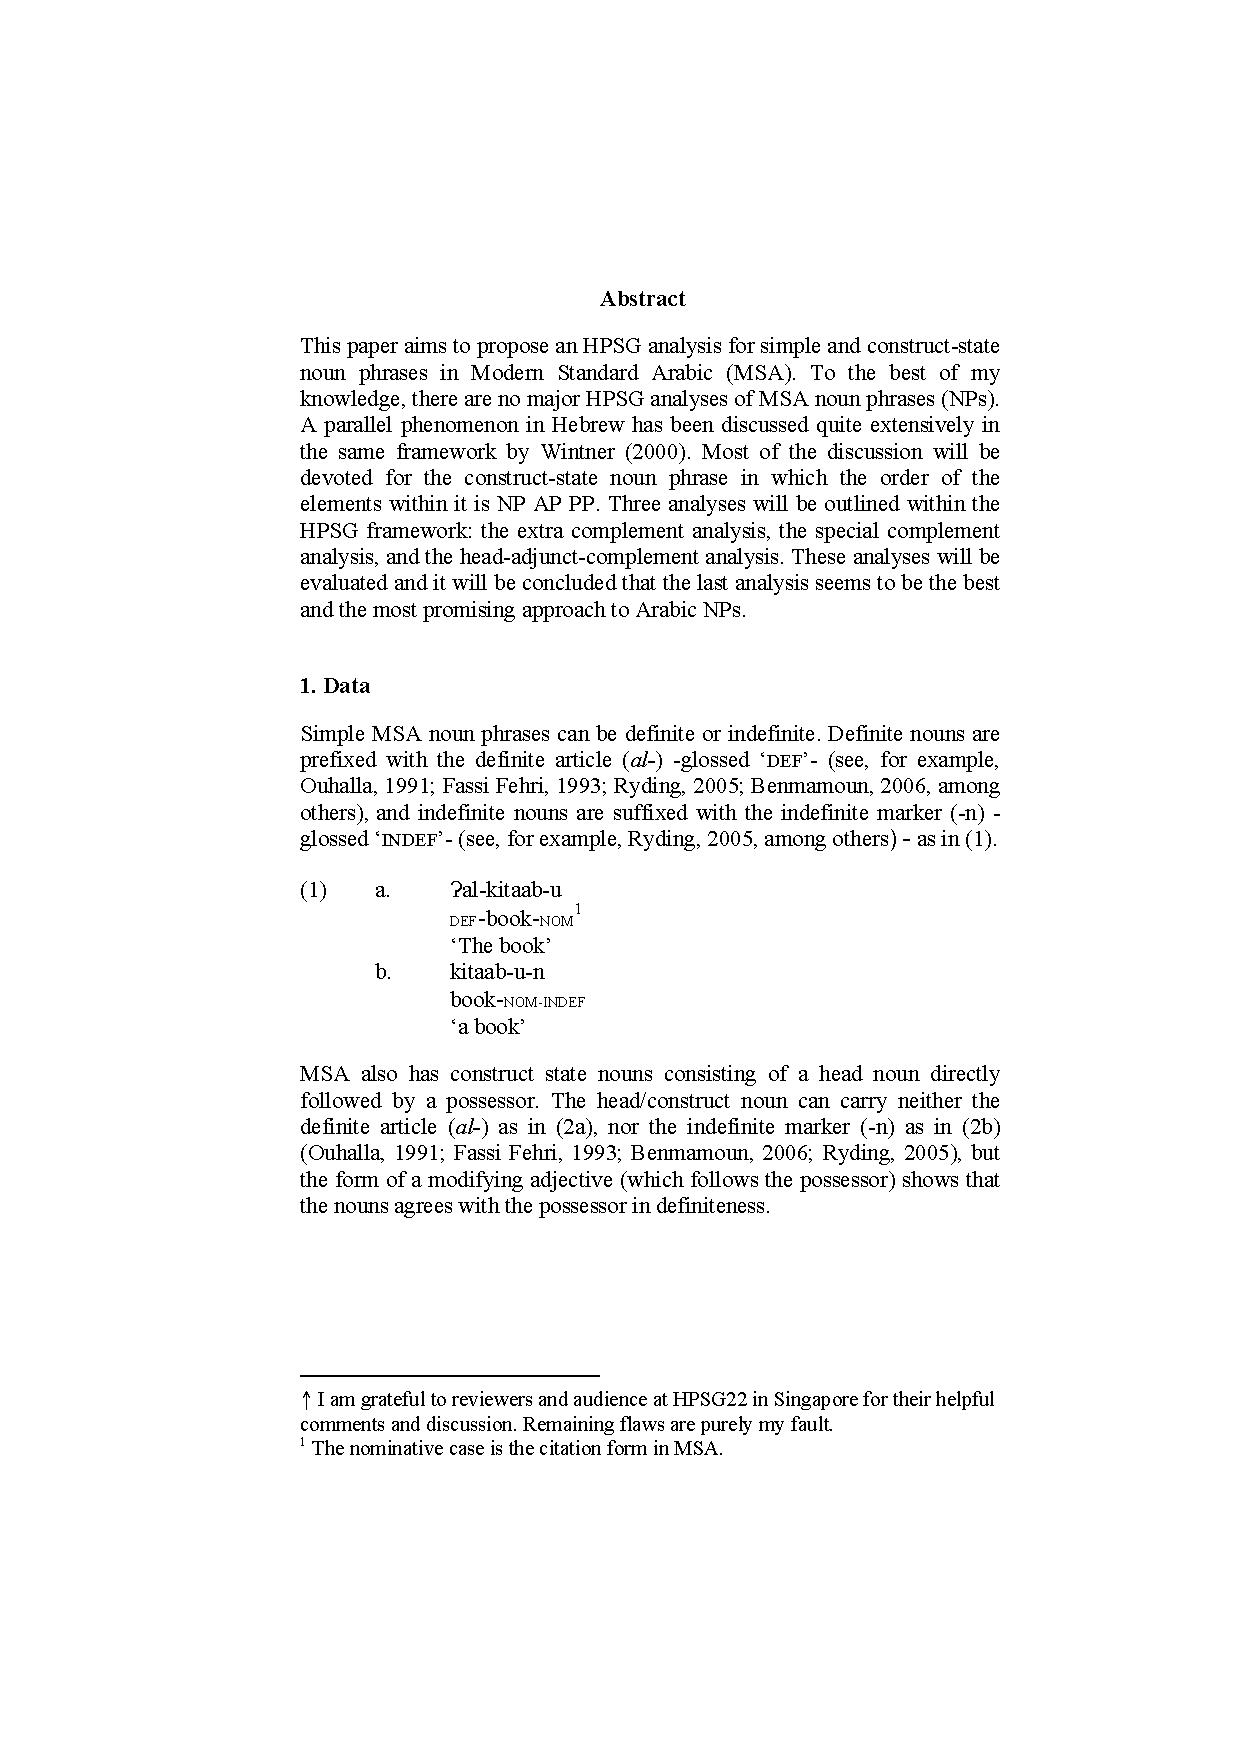
\includepdf[pages=-,pagecommand=\thispagestyle{plain}]{Includes/alqurashi.pdf}
        \setcounter{page}{27}
        \phantomsection
        \addcontentsline{toc}{section}{Tali Arad Greshler, Livnat Herzig Sheinfux, Nurit Melnik, Shuly Wintner: Development of Maximally Reusable Grammars: Parallel Development of Hebrew and Arabic Grammars}
\thispagestyle{empty}

\begin{center}
  {\huge\bfseries Development of Maximally Reusable Grammars: Parallel Development of Hebrew and Arabic Grammars\par}

  \bigskip

~\\
\begingroup
\setlength{\leftskip}{0pt plus 1fill}
\setlength{\rightskip}{0pt plus 1fill}
\setlength{\parindent}{0pt}
\setlength{\parfillskip}{0pt}
  \formatauthor{Tali Arad Greshler}{\begin{tabular}{@{}c@{}}University of Haifa\end{tabular}}
\formatauthor{Livnat Herzig Sheinfux}{\begin{tabular}{@{}c@{}}University of Haifa\end{tabular}}
\formatauthor{Nurit Melnik}{\begin{tabular}{@{}c@{}}The Open University of Israel\end{tabular}}
\formatauthor{Shuly Wintner}{\begin{tabular}{@{}c@{}}University of Haifa\end{tabular}}

\par\endgroup

  \vspace*{8ex}

  Proceedings of the 22nd International Conference on\par Head-Driven Phrase Structure Grammar

  \bigskip

  Nanyang Technological University (NTU), Singapore

  \medskip

  Stefan Müller (Editor)

  \medskip

  2015

  \medskip

  CSLI Publications

  \medskip

  pages 27--40

  \medskip

  \url{http://csli-publications.stanford.edu/HPSG/2015}
\end{center}
\vfill

\noindent



\vfill
\noindent
% APA Style
Arad Greshler, Tali, Herzig Sheinfux, Livnat, Melnik, Nurit, \& Wintner, Shuly. 2015. Development of Maximally Reusable Grammars: Parallel Development of Hebrew and Arabic Grammars. In Müller, Stefan (Ed.), \emph{{Proceedings of the 22nd International Conference on Head-Driven Phrase Structure Grammar, Nanyang Technological University (NTU), Singapore}}, 27--40. Stanford,
CA: CSLI Publications. \hfill\href{http://creativecommons.org/licenses/by/4.0/}{\includegraphics[height=.75em]{Includes/ccby.eps}}

\newpage
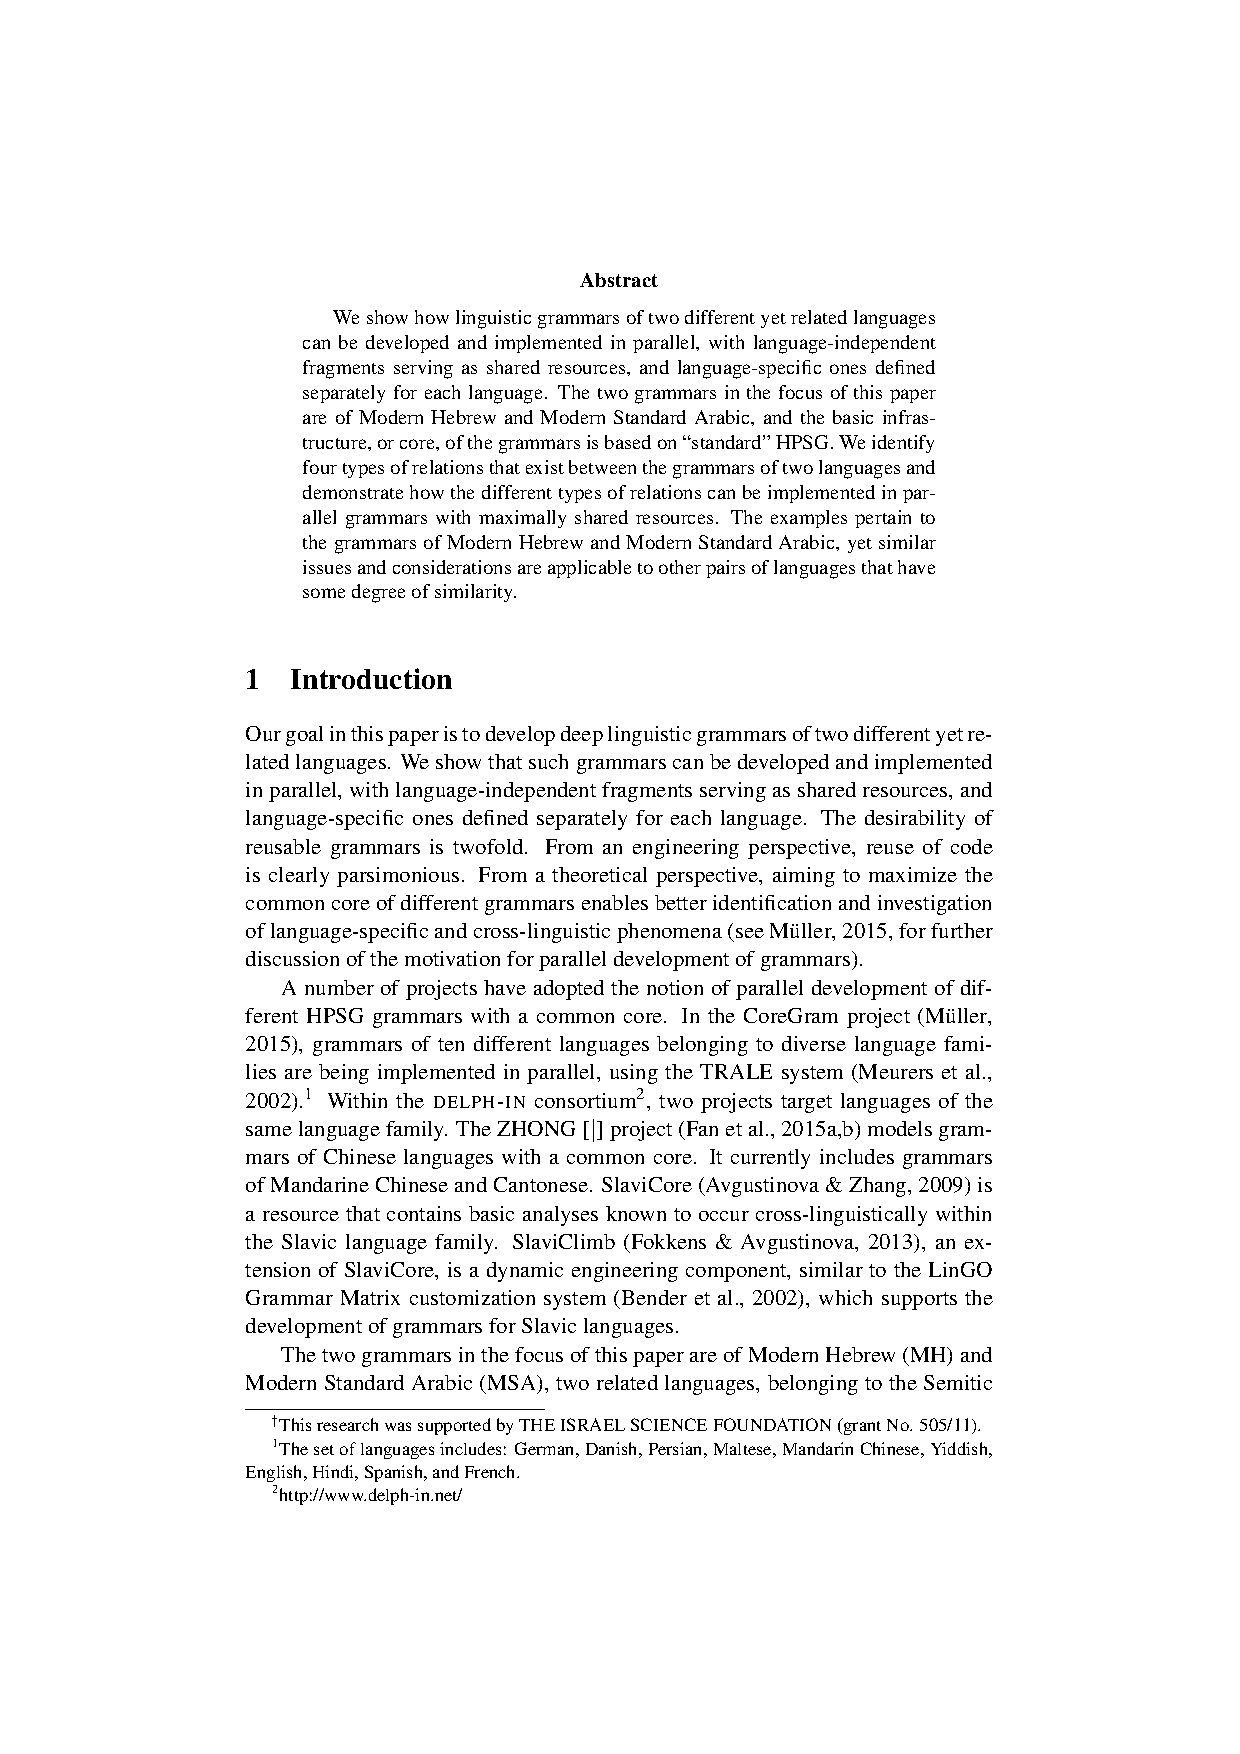
\includepdf[pages=-,pagecommand=\thispagestyle{plain}]{Includes/ahmw.pdf}
        \setcounter{page}{41}
        \phantomsection
        \addcontentsline{toc}{section}{Doug Arnold, Andrew Spencer: A Constructional Analysis for the Skeptical}
\thispagestyle{empty}

\begin{center}
  {\huge\bfseries A Constructional Analysis for the Skeptical\par}

  \bigskip

~\\
\begingroup
\setlength{\leftskip}{0pt plus 1fill}
\setlength{\rightskip}{0pt plus 1fill}
\setlength{\parindent}{0pt}
\setlength{\parfillskip}{0pt}
  \formatauthor{Doug Arnold}{\begin{tabular}{@{}c@{}}University of Essex\end{tabular}}
\formatauthor{Andrew Spencer}{\begin{tabular}{@{}c@{}}University of Essex\end{tabular}}

\par\endgroup

  \vspace*{8ex}

  Proceedings of the 22nd International Conference on\par Head-Driven Phrase Structure Grammar

  \bigskip

  Nanyang Technological University (NTU), Singapore

  \medskip

  Stefan Müller (Editor)

  \medskip

  2015

  \medskip

  CSLI Publications

  \medskip

  pages 41--60

  \medskip

  \url{http://csli-publications.stanford.edu/HPSG/2015}
\end{center}
\vfill

\noindent



\vfill
\noindent
% APA Style
Arnold, Doug, \& Spencer, Andrew. 2015. A Constructional Analysis for the Skeptical. In Müller, Stefan (Ed.), \emph{{Proceedings of the 22nd International Conference on Head-Driven Phrase Structure Grammar, Nanyang Technological University (NTU), Singapore}}, 41--60. Stanford,
CA: CSLI Publications. \hfill\href{http://creativecommons.org/licenses/by/4.0/}{\includegraphics[height=.75em]{Includes/ccby.eps}}

\newpage
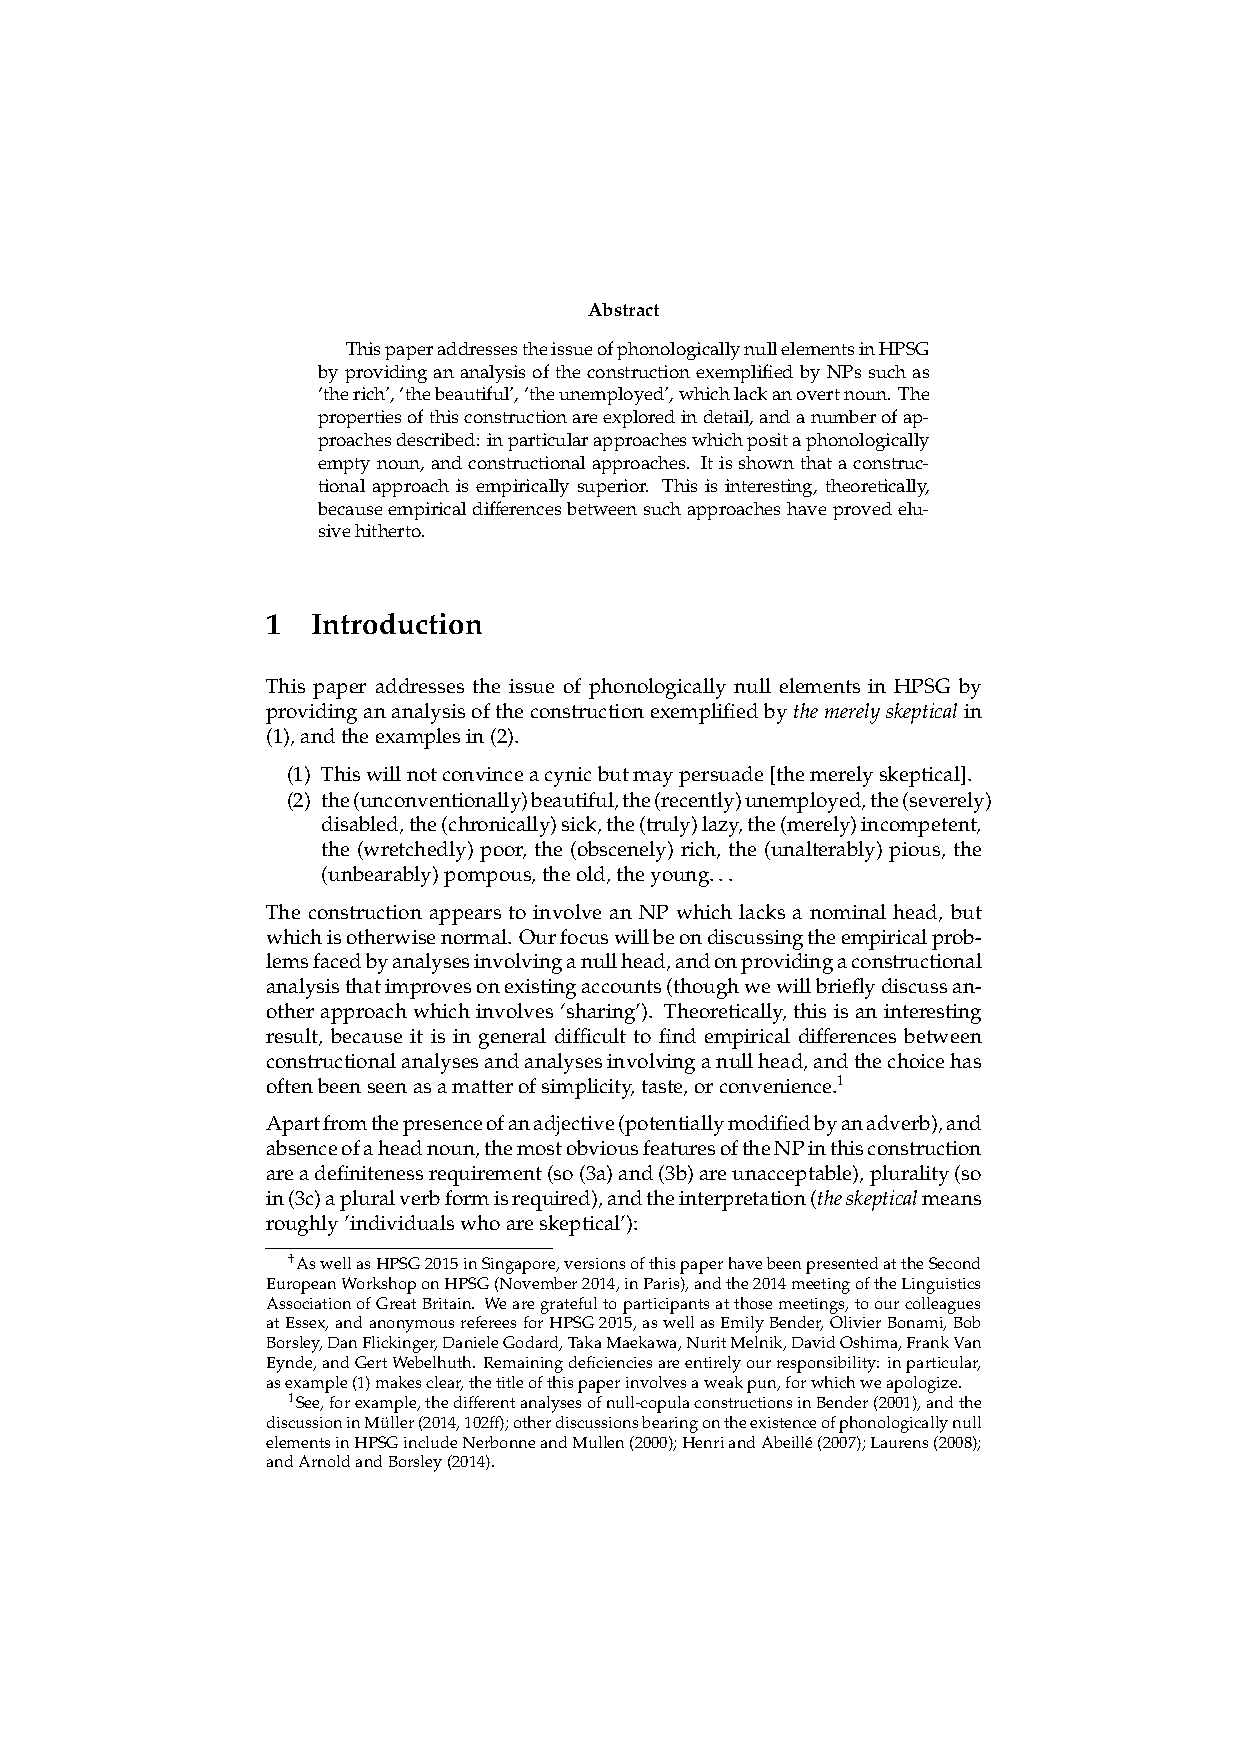
\includepdf[pages=-,pagecommand=\thispagestyle{plain}]{Includes/arnold-spencer.pdf}
        \setcounter{page}{61}
        \phantomsection
        \addcontentsline{toc}{section}{Francis Bond, Jia Qian Ho, Dan Flickinger: Feeling our way to an analysis of English possessed idioms}
\thispagestyle{empty}

\begin{center}
  {\huge\bfseries Feeling our way to an analysis of English possessed idioms\par}

  \bigskip

~\\
\begingroup
\setlength{\leftskip}{0pt plus 1fill}
\setlength{\rightskip}{0pt plus 1fill}
\setlength{\parindent}{0pt}
\setlength{\parfillskip}{0pt}
  \formatauthor{Francis Bond}{\begin{tabular}{@{}c@{}}Nanyang Technological University\end{tabular}}
\formatauthor{Jia Qian Ho}{\begin{tabular}{@{}c@{}}NanyanUniversity\end{tabular}}
\formatauthor{Dan Flickinger}{\begin{tabular}{@{}c@{}}Stanford University\end{tabular}}

\par\endgroup

  \vspace*{8ex}

  Proceedings of the 22nd International Conference on\par Head-Driven Phrase Structure Grammar

  \bigskip

  Nanyang Technological University (NTU), Singapore

  \medskip

  Stefan Müller (Editor)

  \medskip

  2015

  \medskip

  CSLI Publications

  \medskip

  pages 61--74

  \medskip

  \url{http://csli-publications.stanford.edu/HPSG/2015}
\end{center}
\vfill

\noindent



\vfill
\noindent
% APA Style
Bond, Francis, Ho, Jia Qian, \& Flickinger, Dan. 2015. Feeling our way to an analysis of English possessed idioms. In Müller, Stefan (Ed.), \emph{{Proceedings of the 22nd International Conference on Head-Driven Phrase Structure Grammar, Nanyang Technological University (NTU), Singapore}}, 61--74. Stanford,
CA: CSLI Publications. \hfill\href{http://creativecommons.org/licenses/by/4.0/}{\includegraphics[height=.75em]{Includes/ccby.eps}}

\newpage
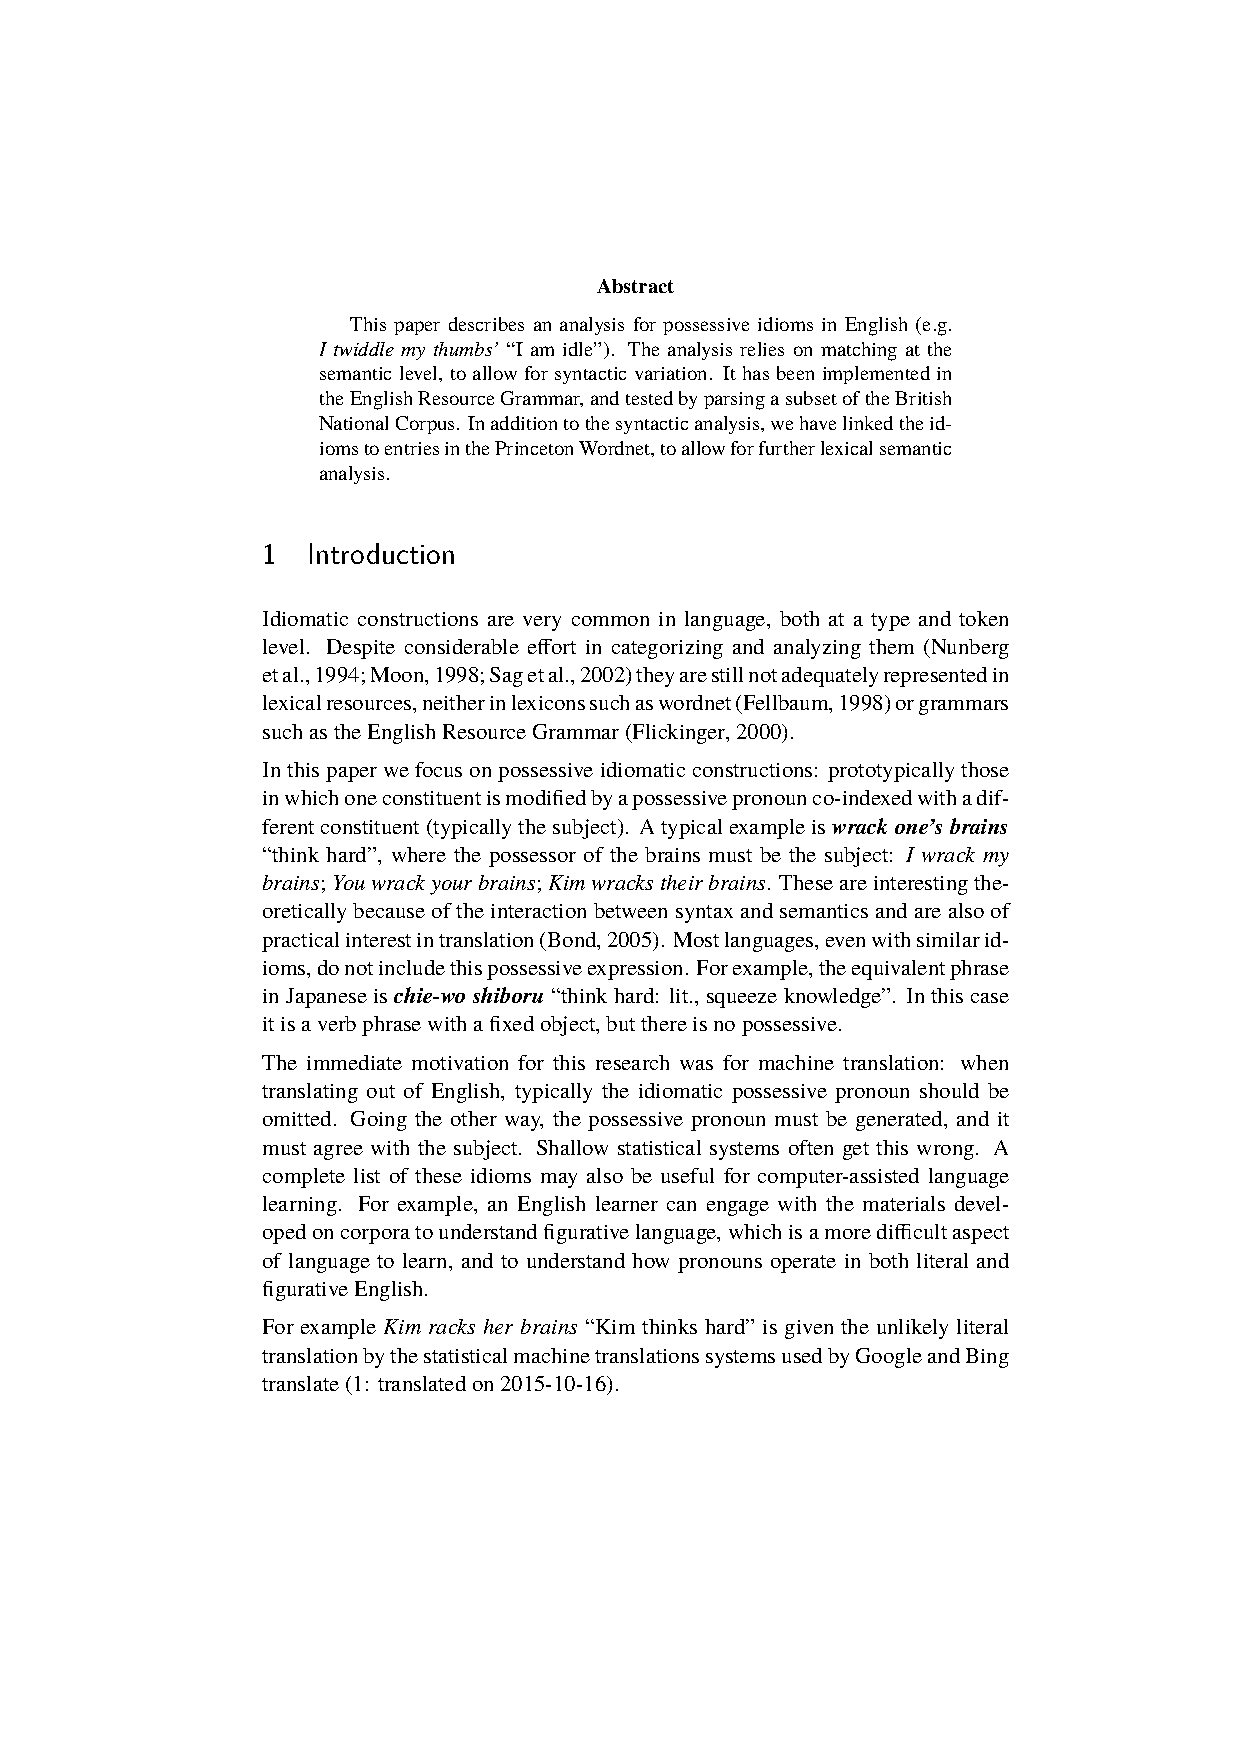
\includepdf[pages=-,pagecommand=\thispagestyle{plain}]{Includes/bhf.pdf}
        \setcounter{page}{75}
        \phantomsection
        \addcontentsline{toc}{section}{Guy Emerson, Ann Copestake: Lacking Integrity: HPSG as a Morphosyntactic Theory}
\thispagestyle{empty}

\begin{center}
  {\huge\bfseries Lacking Integrity: HPSG as a Morphosyntactic Theory\par}

  \bigskip

~\\
\begingroup
\setlength{\leftskip}{0pt plus 1fill}
\setlength{\rightskip}{0pt plus 1fill}
\setlength{\parindent}{0pt}
\setlength{\parfillskip}{0pt}
  \formatauthor{Guy Emerson}{\begin{tabular}{@{}c@{}}University of Cambridge\end{tabular}}
\formatauthor{Ann Copestake}{\begin{tabular}{@{}c@{}}University of Cambridge\end{tabular}}

\par\endgroup

  \vspace*{8ex}

  Proceedings of the 22nd International Conference on\par Head-Driven Phrase Structure Grammar

  \bigskip

  Nanyang Technological University (NTU), Singapore

  \medskip

  Stefan Müller (Editor)

  \medskip

  2015

  \medskip

  CSLI Publications

  \medskip

  pages 75--95

  \medskip

  \url{http://csli-publications.stanford.edu/HPSG/2015}
\end{center}
\vfill

\noindent



\vfill
\noindent
% APA Style
Emerson, Guy, \& Copestake, Ann. 2015. Lacking Integrity: HPSG as a Morphosyntactic Theory. In Müller, Stefan (Ed.), \emph{{Proceedings of the 22nd International Conference on Head-Driven Phrase Structure Grammar, Nanyang Technological University (NTU), Singapore}}, 75--95. Stanford,
CA: CSLI Publications. \hfill\href{http://creativecommons.org/licenses/by/4.0/}{\includegraphics[height=.75em]{Includes/ccby.eps}}

\newpage
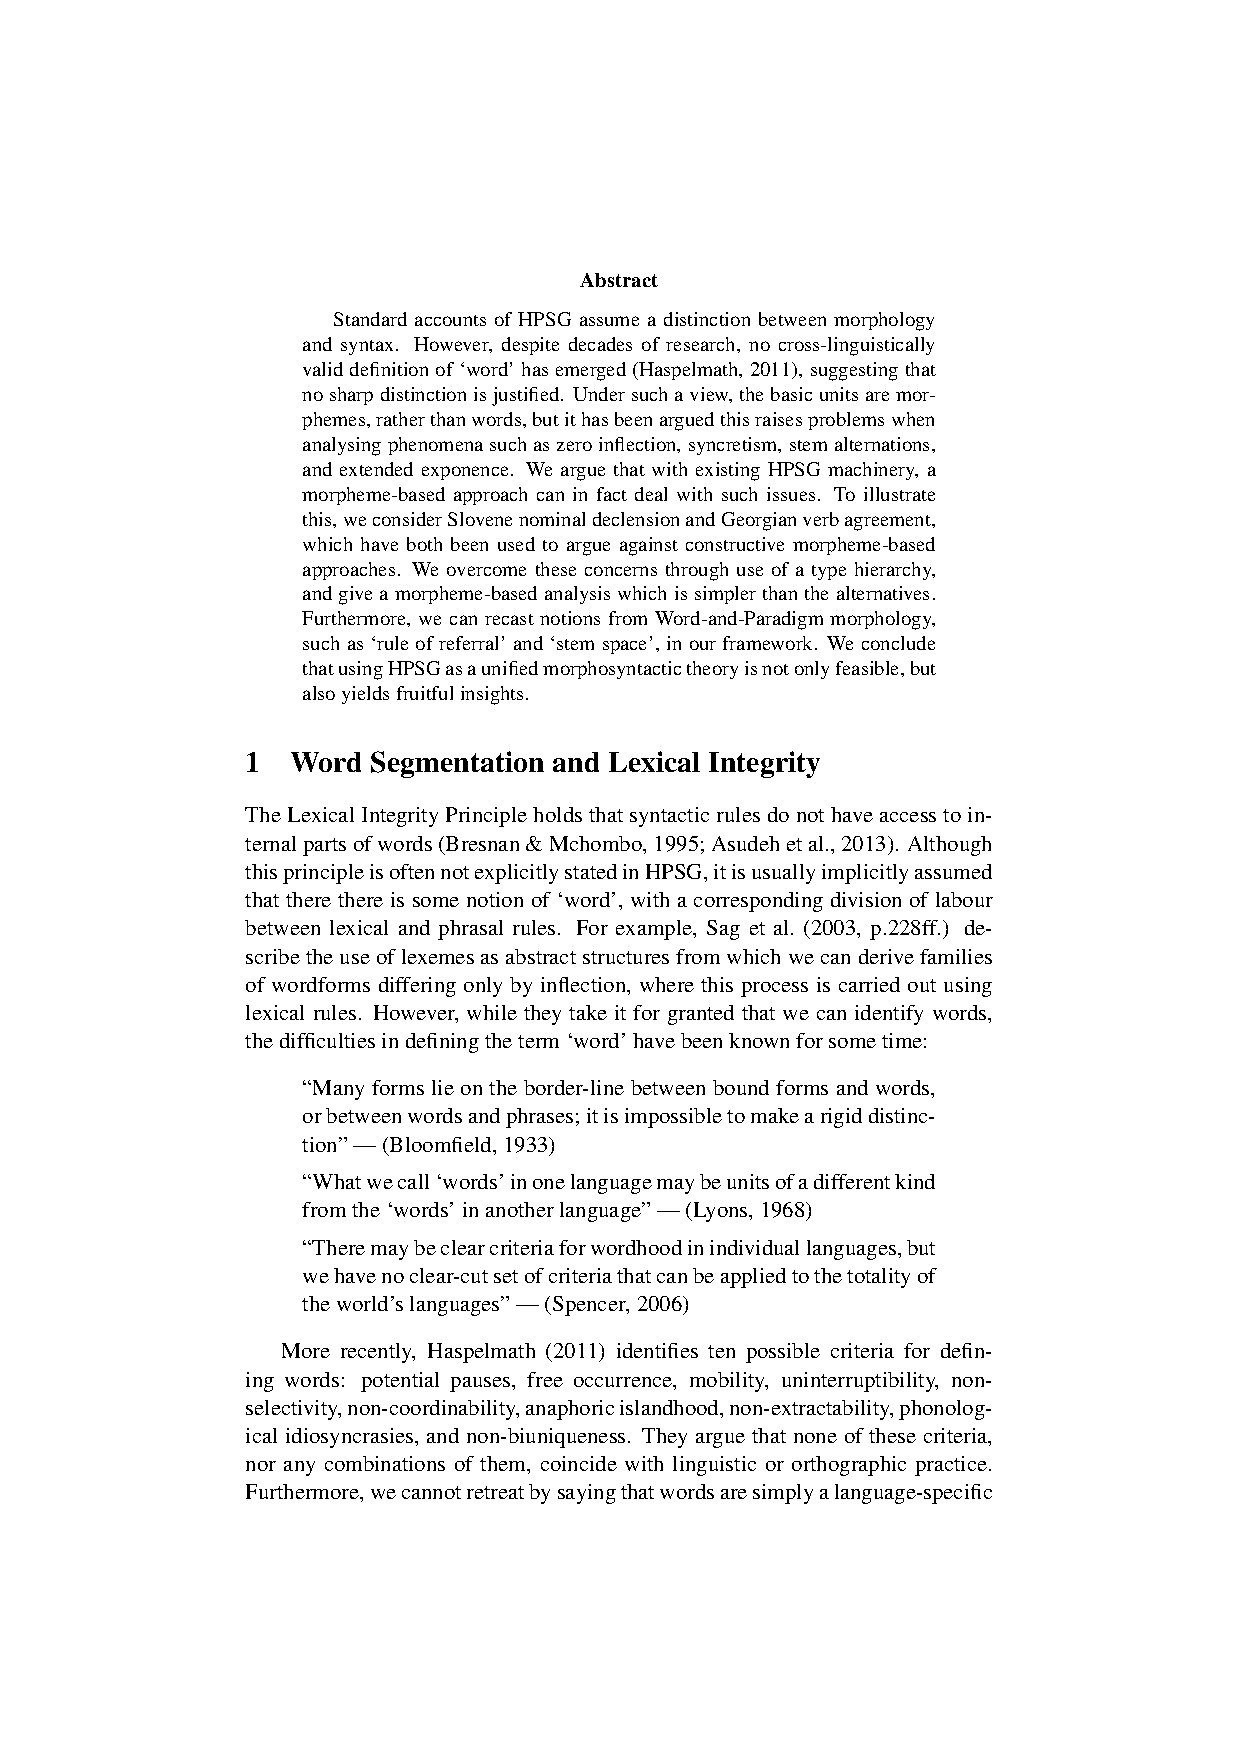
\includepdf[pages=-,pagecommand=\thispagestyle{plain}]{Includes/emerson-copestake.pdf}
        \setcounter{page}{96}
        \phantomsection
        \addcontentsline{toc}{section}{Zhenzhen Fan, Sanghoun Song, Francis Bond: Building Zhong, a Chinese HPSG Shared-Grammar}
\thispagestyle{empty}

\begin{center}
  {\huge\bfseries Building Zhong, a Chinese HPSG Shared-Grammar\par}

  \bigskip

~\\
\begingroup
\setlength{\leftskip}{0pt plus 1fill}
\setlength{\rightskip}{0pt plus 1fill}
\setlength{\parindent}{0pt}
\setlength{\parfillskip}{0pt}
  \formatauthor{Zhenzhen Fan}{\begin{tabular}{@{}c@{}}National University of Singapore\end{tabular}}
\formatauthor{Sanghoun Song}{\begin{tabular}{@{}c@{}}Incheon National University\end{tabular}}
\formatauthor{Francis Bond}{\begin{tabular}{@{}c@{}}Nanyang Technological University\end{tabular}}

\par\endgroup

  \vspace*{8ex}

  Proceedings of the 22nd International Conference on\par Head-Driven Phrase Structure Grammar

  \bigskip

  Nanyang Technological University (NTU), Singapore

  \medskip

  Stefan Müller (Editor)

  \medskip

  2015

  \medskip

  CSLI Publications

  \medskip

  pages 96--109

  \medskip

  \url{http://csli-publications.stanford.edu/HPSG/2015}
\end{center}
\vfill

\noindent



\vfill
\noindent
% APA Style
Fan, Zhenzhen, Song, Sanghoun, \& Bond, Francis. 2015. Building Zhong, a Chinese HPSG Shared-Grammar. In Müller, Stefan (Ed.), \emph{{Proceedings of the 22nd International Conference on Head-Driven Phrase Structure Grammar, Nanyang Technological University (NTU), Singapore}}, 96--109. Stanford,
CA: CSLI Publications. \hfill\href{http://creativecommons.org/licenses/by/4.0/}{\includegraphics[height=.75em]{Includes/ccby.eps}}

\newpage
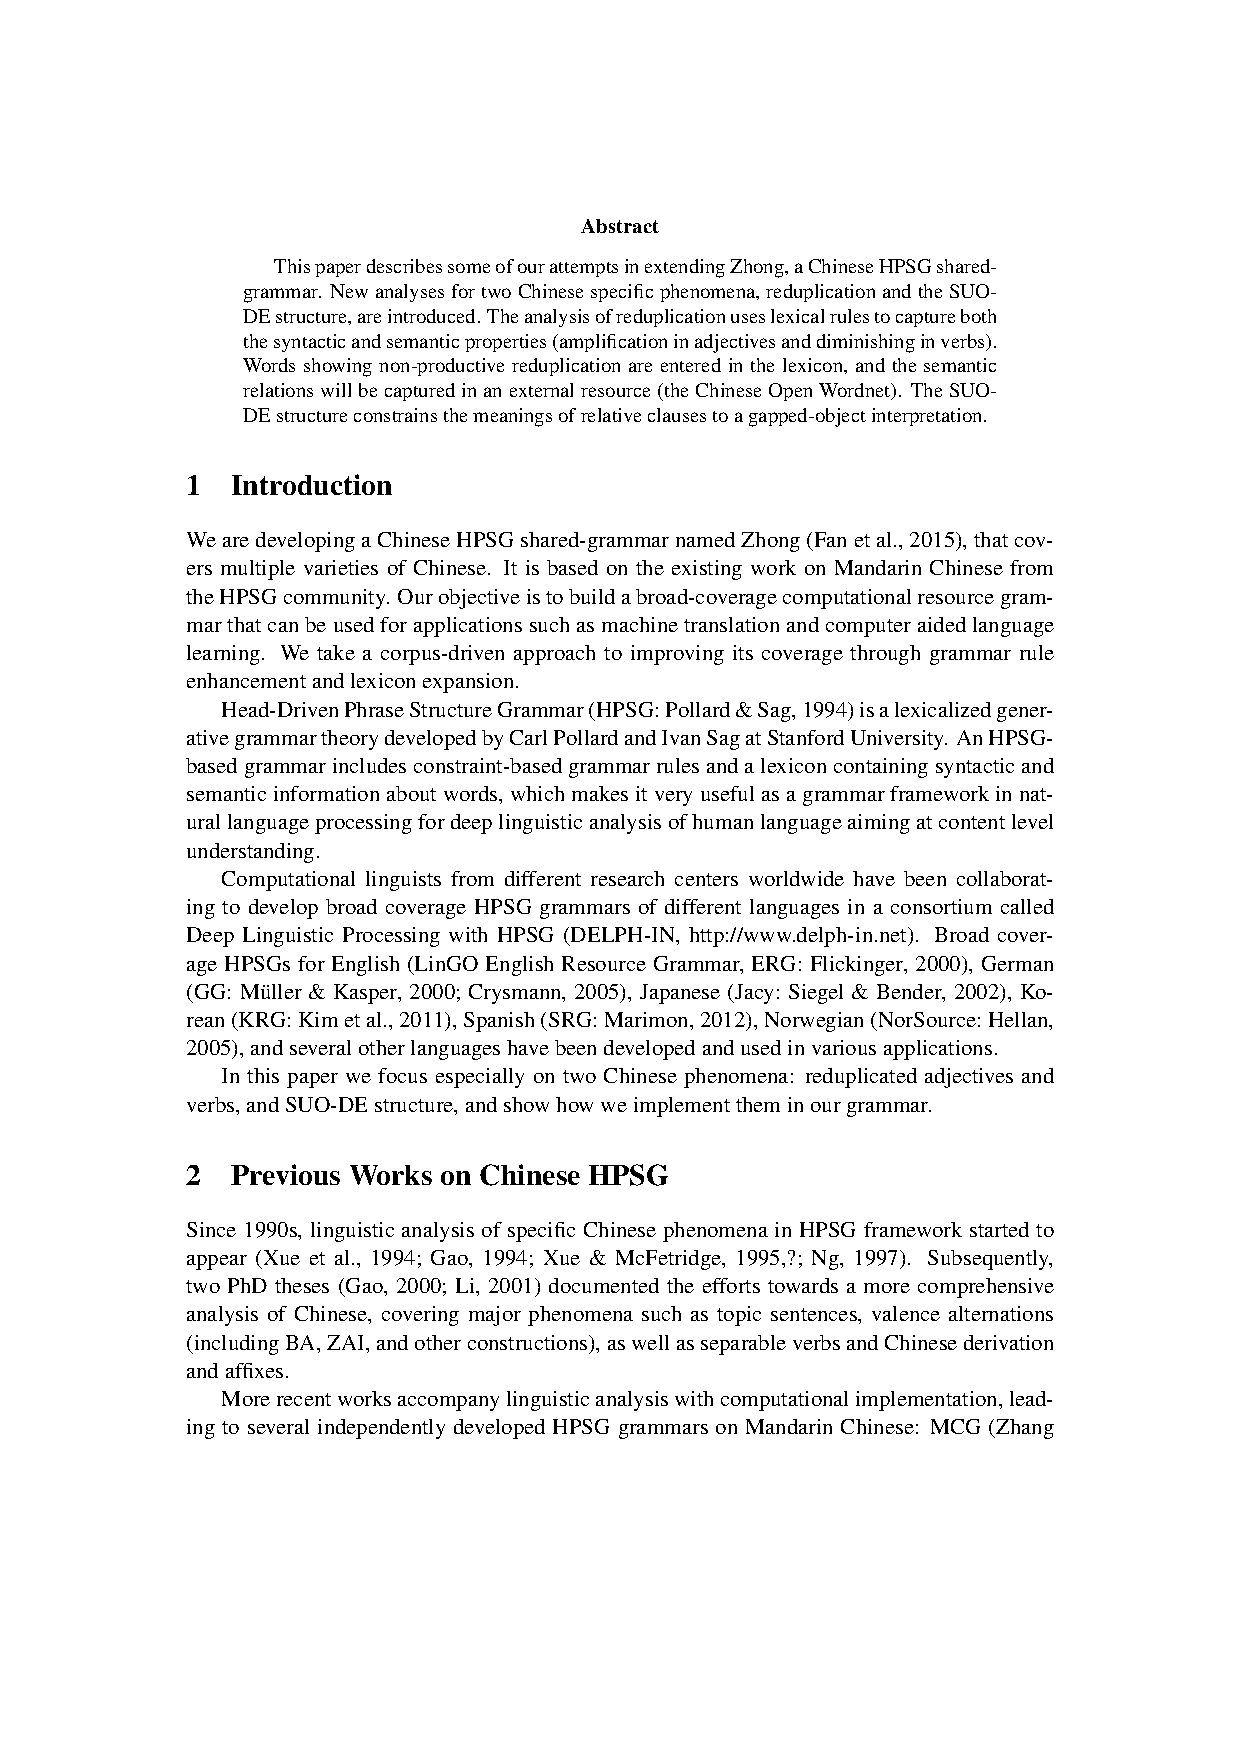
\includepdf[pages=-,pagecommand=\thispagestyle{plain}]{Includes/fsb.pdf}
        \setcounter{page}{110}
        \phantomsection
        \addcontentsline{toc}{section}{Petter Haugereid: Unique lexical entries in a subconstructional grammar}
\thispagestyle{empty}

\begin{center}
  {\huge\bfseries Unique lexical entries in a subconstructional grammar\par}

  \bigskip

~\\
\begingroup
\setlength{\leftskip}{0pt plus 1fill}
\setlength{\rightskip}{0pt plus 1fill}
\setlength{\parindent}{0pt}
\setlength{\parfillskip}{0pt}
  \formatauthor{Petter Haugereid}{\begin{tabular}{@{}c@{}}Bergen University College\end{tabular}}

\par\endgroup

  \vspace*{8ex}

  Proceedings of the 22nd International Conference on\par Head-Driven Phrase Structure Grammar

  \bigskip

  Nanyang Technological University (NTU), Singapore

  \medskip

  Stefan Müller (Editor)

  \medskip

  2015

  \medskip

  CSLI Publications

  \medskip

  pages 110--121

  \medskip

  \url{http://csli-publications.stanford.edu/HPSG/2015}
\end{center}
\vfill

\noindent



\vfill
\noindent
% APA Style
Haugereid, Petter. 2015. Unique lexical entries in a subconstructional grammar. In Müller, Stefan (Ed.), \emph{{Proceedings of the 22nd International Conference on Head-Driven Phrase Structure Grammar, Nanyang Technological University (NTU), Singapore}}, 110--121. Stanford,
CA: CSLI Publications. \hfill\href{http://creativecommons.org/licenses/by/4.0/}{\includegraphics[height=.75em]{Includes/ccby.eps}}

\newpage
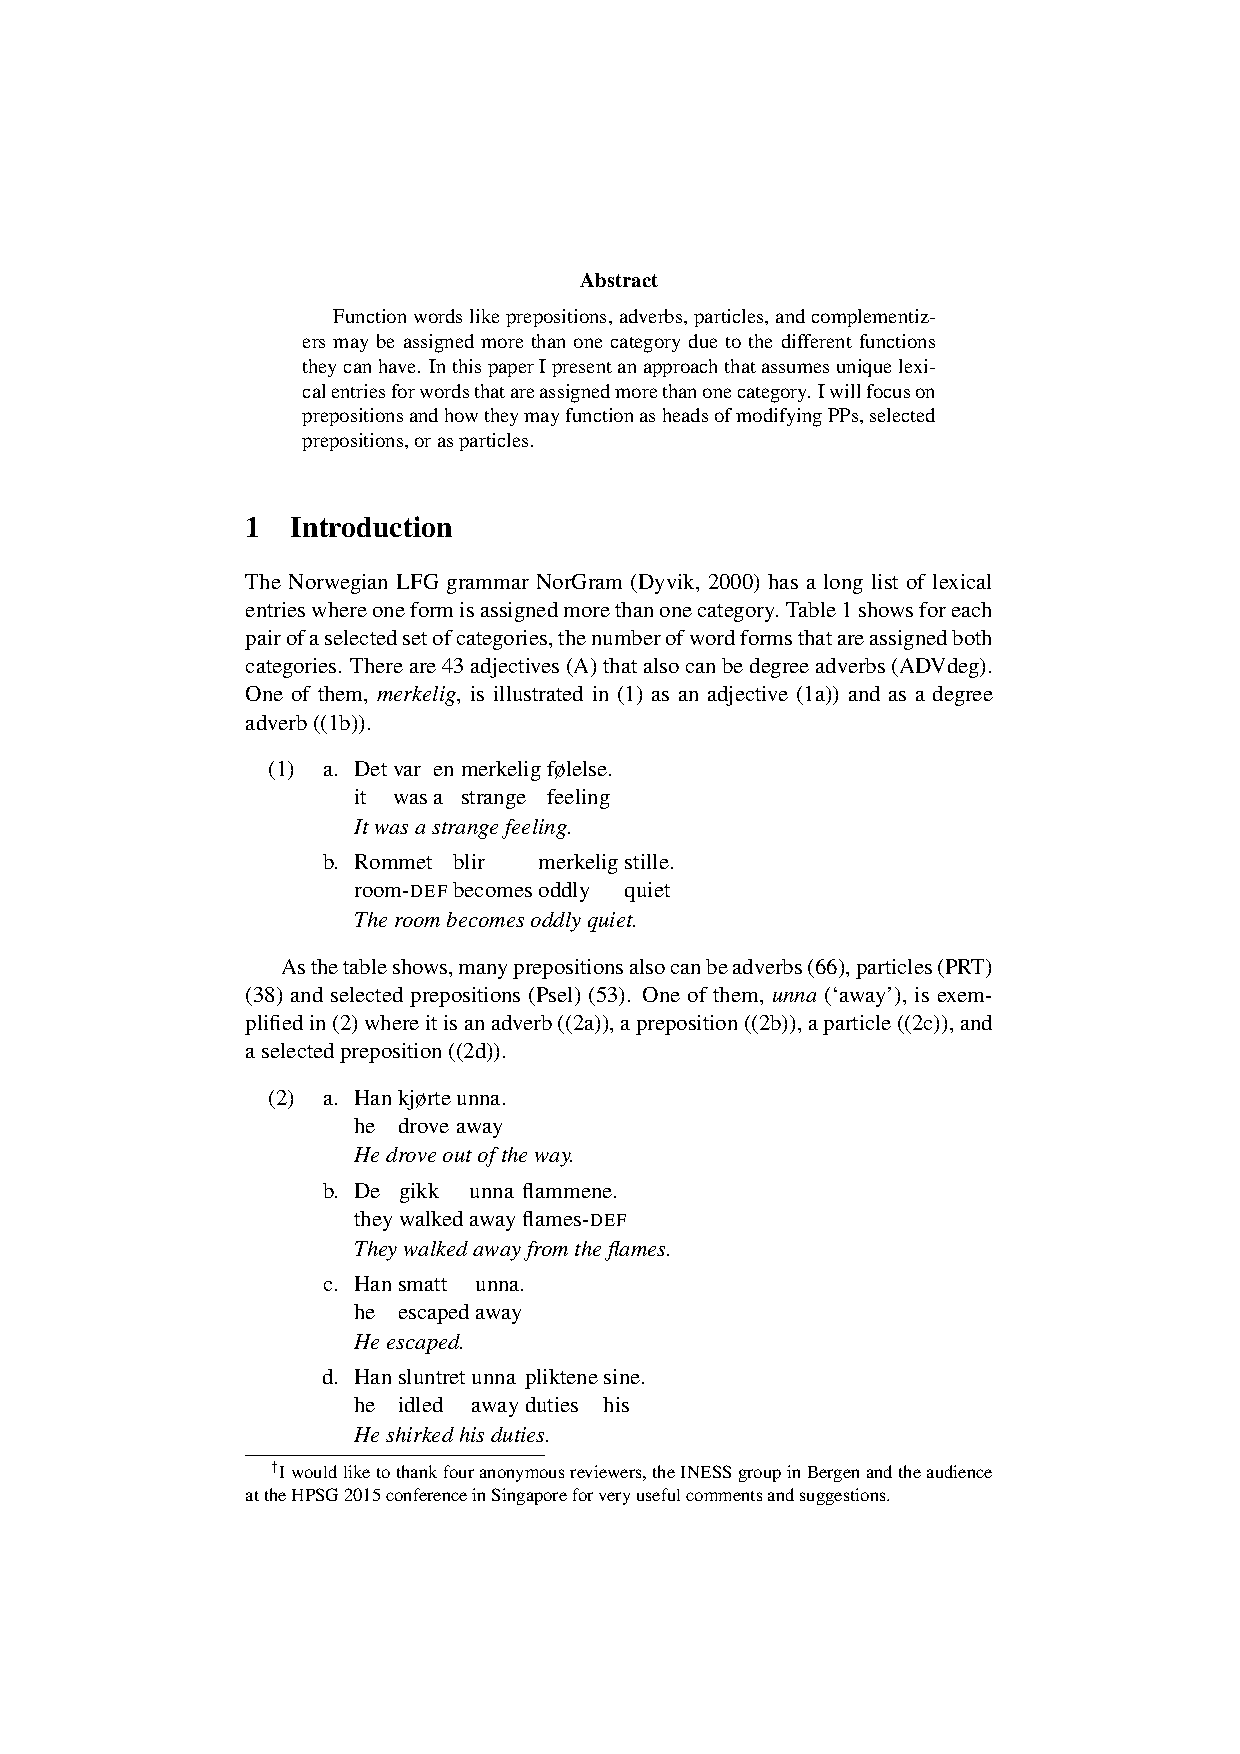
\includepdf[pages=-,pagecommand=\thispagestyle{plain}]{Includes/haugereid.pdf}
        \setcounter{page}{122}
        \phantomsection
        \addcontentsline{toc}{section}{Livnat Herzig Sheinfux, Tali Arad Greshler, Nurit Melnik, Shuly Wintner: Hebrew Verbal Multi-Word Expressions}
\thispagestyle{empty}

\begin{center}
  {\huge\bfseries Hebrew Verbal Multi-Word Expressions\par}

  \bigskip

~\\
\begingroup
\setlength{\leftskip}{0pt plus 1fill}
\setlength{\rightskip}{0pt plus 1fill}
\setlength{\parindent}{0pt}
\setlength{\parfillskip}{0pt}
  \formatauthor{Livnat Herzig Sheinfux}{\begin{tabular}{@{}c@{}}University of Haifa\end{tabular}}
\formatauthor{Tali Arad Greshler}{\begin{tabular}{@{}c@{}}University of Haifa\end{tabular}}
\formatauthor{Nurit Melnik}{\begin{tabular}{@{}c@{}}The Open University of Israel\end{tabular}}
\formatauthor{Shuly Wintner}{\begin{tabular}{@{}c@{}}University of Haifa\end{tabular}}

\par\endgroup

  \vspace*{8ex}

  Proceedings of the 22nd International Conference on\par Head-Driven Phrase Structure Grammar

  \bigskip

  Nanyang Technological University (NTU), Singapore

  \medskip

  Stefan Müller (Editor)

  \medskip

  2015

  \medskip

  CSLI Publications

  \medskip

  pages 122--135

  \medskip

  \url{http://csli-publications.stanford.edu/HPSG/2015}
\end{center}
\vfill

\noindent



\vfill
\noindent
% APA Style
Herzig Sheinfux, Livnat, Arad Greshler, Tali, Melnik, Nurit, \& Wintner, Shuly. 2015. Hebrew Verbal Multi-Word Expressions. In Müller, Stefan (Ed.), \emph{{Proceedings of the 22nd International Conference on Head-Driven Phrase Structure Grammar, Nanyang Technological University (NTU), Singapore}}, 122--135. Stanford,
CA: CSLI Publications. \hfill\href{http://creativecommons.org/licenses/by/4.0/}{\includegraphics[height=.75em]{Includes/ccby.eps}}

\newpage
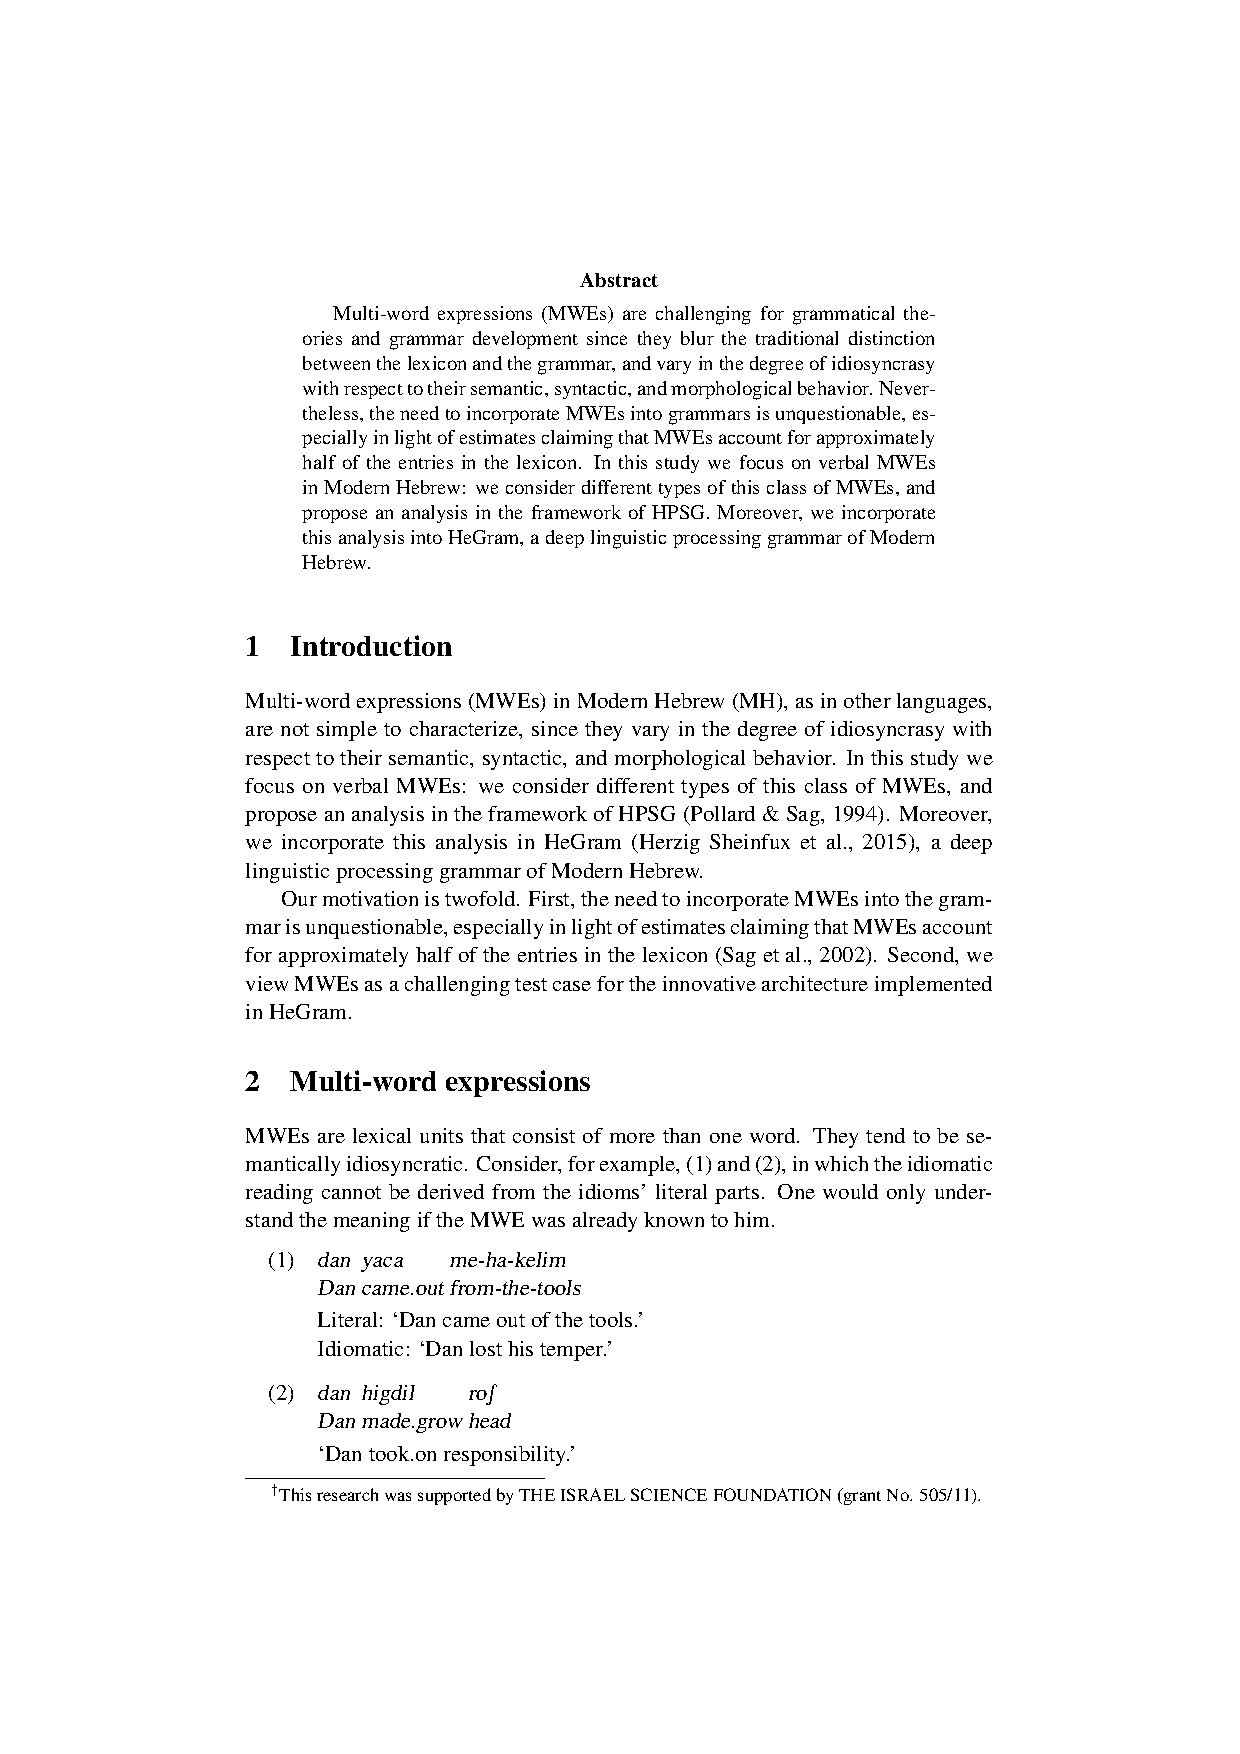
\includepdf[pages=-,pagecommand=\thispagestyle{plain}]{Includes/hamw.pdf}
        \setcounter{page}{136}
        \phantomsection
        \addcontentsline{toc}{section}{Takafumi Maekawa: `Agreement mismatch' between sort/kind/type and the determiner}
\thispagestyle{empty}

\begin{center}
  {\huge\bfseries `Agreement mismatch' between sort/kind/type and the determiner\par}

  \bigskip

~\\
\begingroup
\setlength{\leftskip}{0pt plus 1fill}
\setlength{\rightskip}{0pt plus 1fill}
\setlength{\parindent}{0pt}
\setlength{\parfillskip}{0pt}
  \formatauthor{Takafumi Maekawa}{\begin{tabular}{@{}c@{}}Ryukoku University\end{tabular}}

\par\endgroup

  \vspace*{8ex}

  Proceedings of the 22nd International Conference on\par Head-Driven Phrase Structure Grammar

  \bigskip

  Nanyang Technological University (NTU), Singapore

  \medskip

  Stefan Müller (Editor)

  \medskip

  2015

  \medskip

  CSLI Publications

  \medskip

  pages 136--156

  \medskip

  \url{http://csli-publications.stanford.edu/HPSG/2015}
\end{center}
\vfill

\noindent



\vfill
\noindent
% APA Style
Maekawa, Takafumi. 2015. `Agreement mismatch' between sort/kind/type and the determiner. In Müller, Stefan (Ed.), \emph{{Proceedings of the 22nd International Conference on Head-Driven Phrase Structure Grammar, Nanyang Technological University (NTU), Singapore}}, 136--156. Stanford,
CA: CSLI Publications. \hfill\href{http://creativecommons.org/licenses/by/4.0/}{\includegraphics[height=.75em]{Includes/ccby.eps}}

\newpage
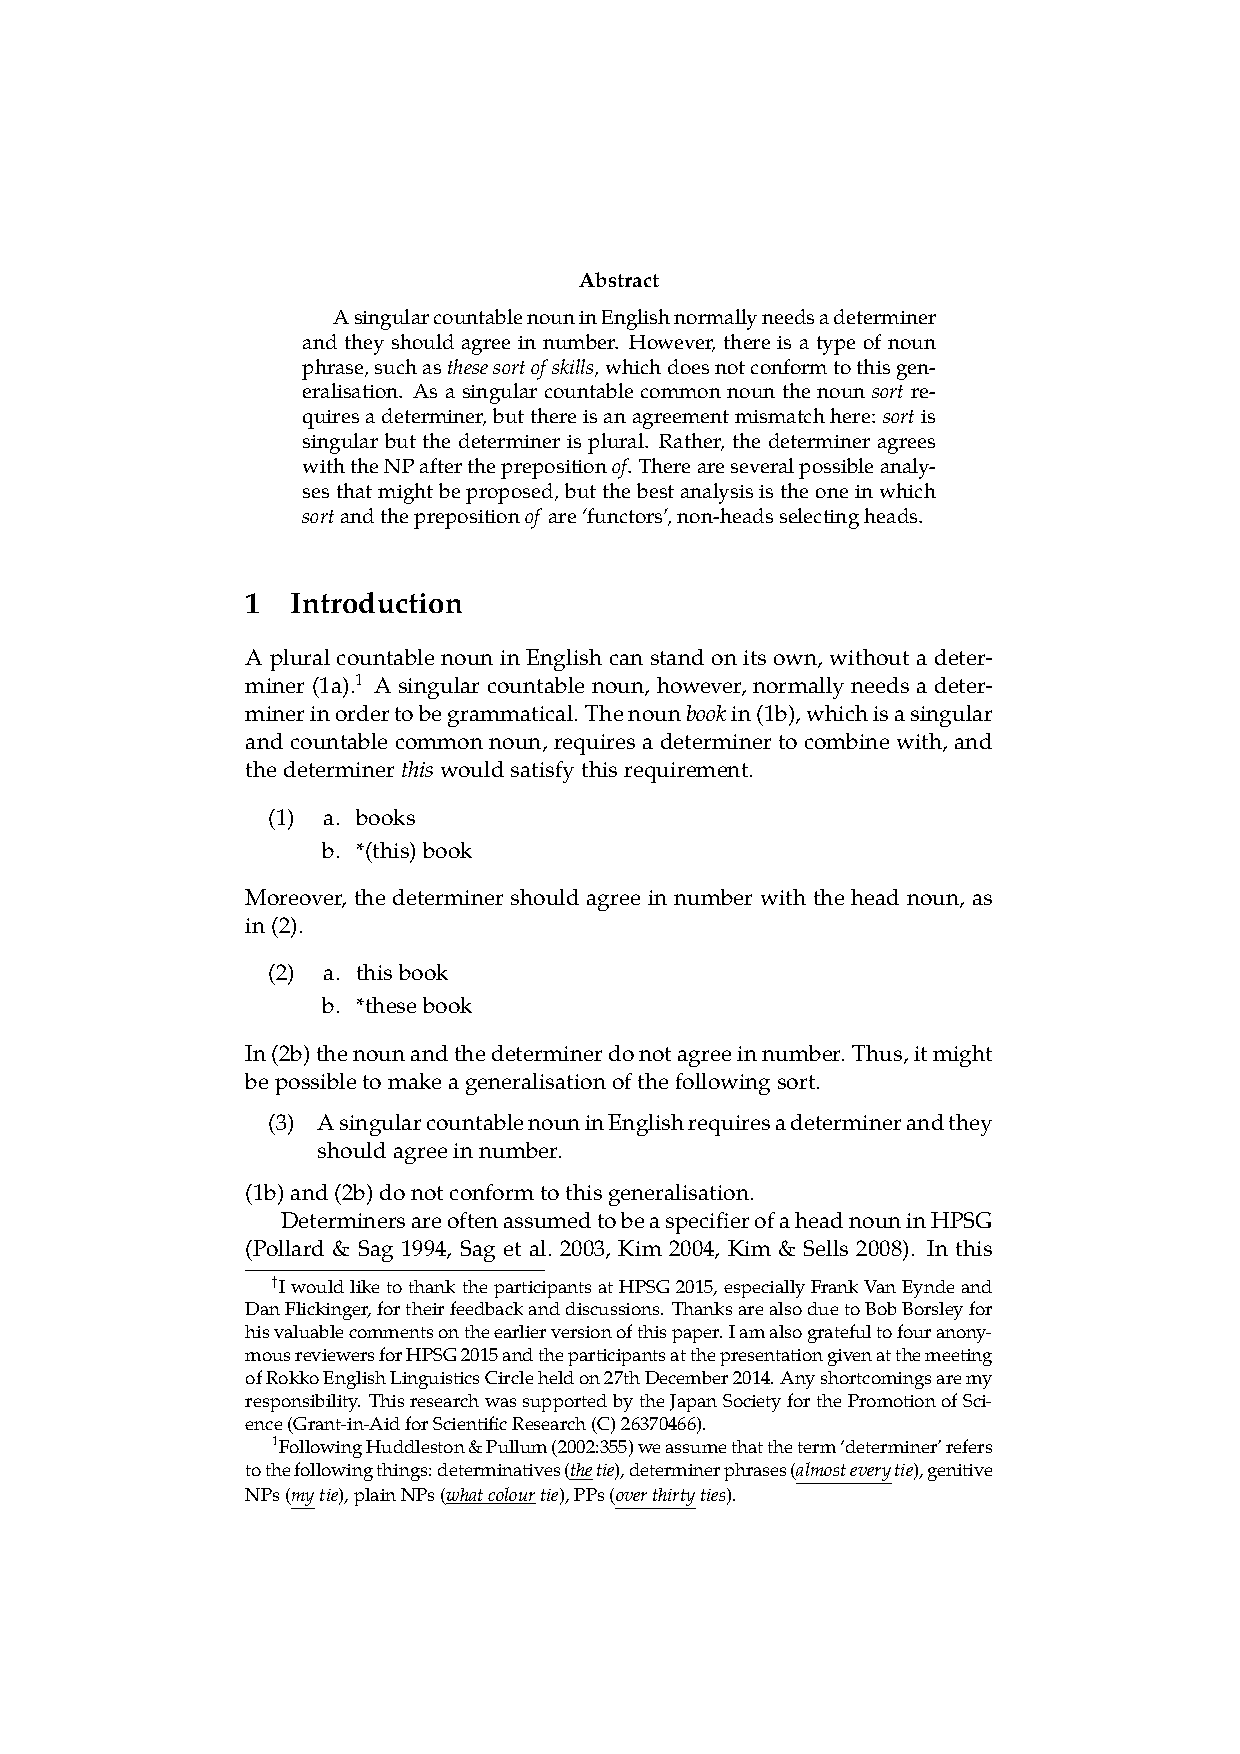
\includepdf[pages=-,pagecommand=\thispagestyle{plain}]{Includes/maekawa.pdf}
        \setcounter{page}{157}
        \phantomsection
        \addcontentsline{toc}{section}{David Y. Oshima: Ellipsis of SAY, THINK, and DO in Japanese subordinate clauses: A constructional analysis}
\thispagestyle{empty}

\begin{center}
  {\huge\bfseries Ellipsis of SAY, THINK, and DO in Japanese subordinate clauses: A constructional analysis\par}

  \bigskip

~\\
\begingroup
\setlength{\leftskip}{0pt plus 1fill}
\setlength{\rightskip}{0pt plus 1fill}
\setlength{\parindent}{0pt}
\setlength{\parfillskip}{0pt}
  \formatauthor{David Y. Oshima}{\begin{tabular}{@{}c@{}}Nagoya University\end{tabular}}

\par\endgroup

  \vspace*{8ex}

  Proceedings of the 22nd International Conference on\par Head-Driven Phrase Structure Grammar

  \bigskip

  Nanyang Technological University (NTU), Singapore

  \medskip

  Stefan Müller (Editor)

  \medskip

  2015

  \medskip

  CSLI Publications

  \medskip

  pages 157--176

  \medskip

  \url{http://csli-publications.stanford.edu/HPSG/2015}
\end{center}
\vfill

\noindent



\vfill
\noindent
% APA Style
Oshima, David Y. 2015. Ellipsis of SAY, THINK, and DO in Japanese subordinate clauses: A constructional analysis. In Müller, Stefan (Ed.), \emph{{Proceedings of the 22nd International Conference on Head-Driven Phrase Structure Grammar, Nanyang Technological University (NTU), Singapore}}, 157--176. Stanford,
CA: CSLI Publications. \hfill\href{http://creativecommons.org/licenses/by/4.0/}{\includegraphics[height=.75em]{Includes/ccby.eps}}

\newpage
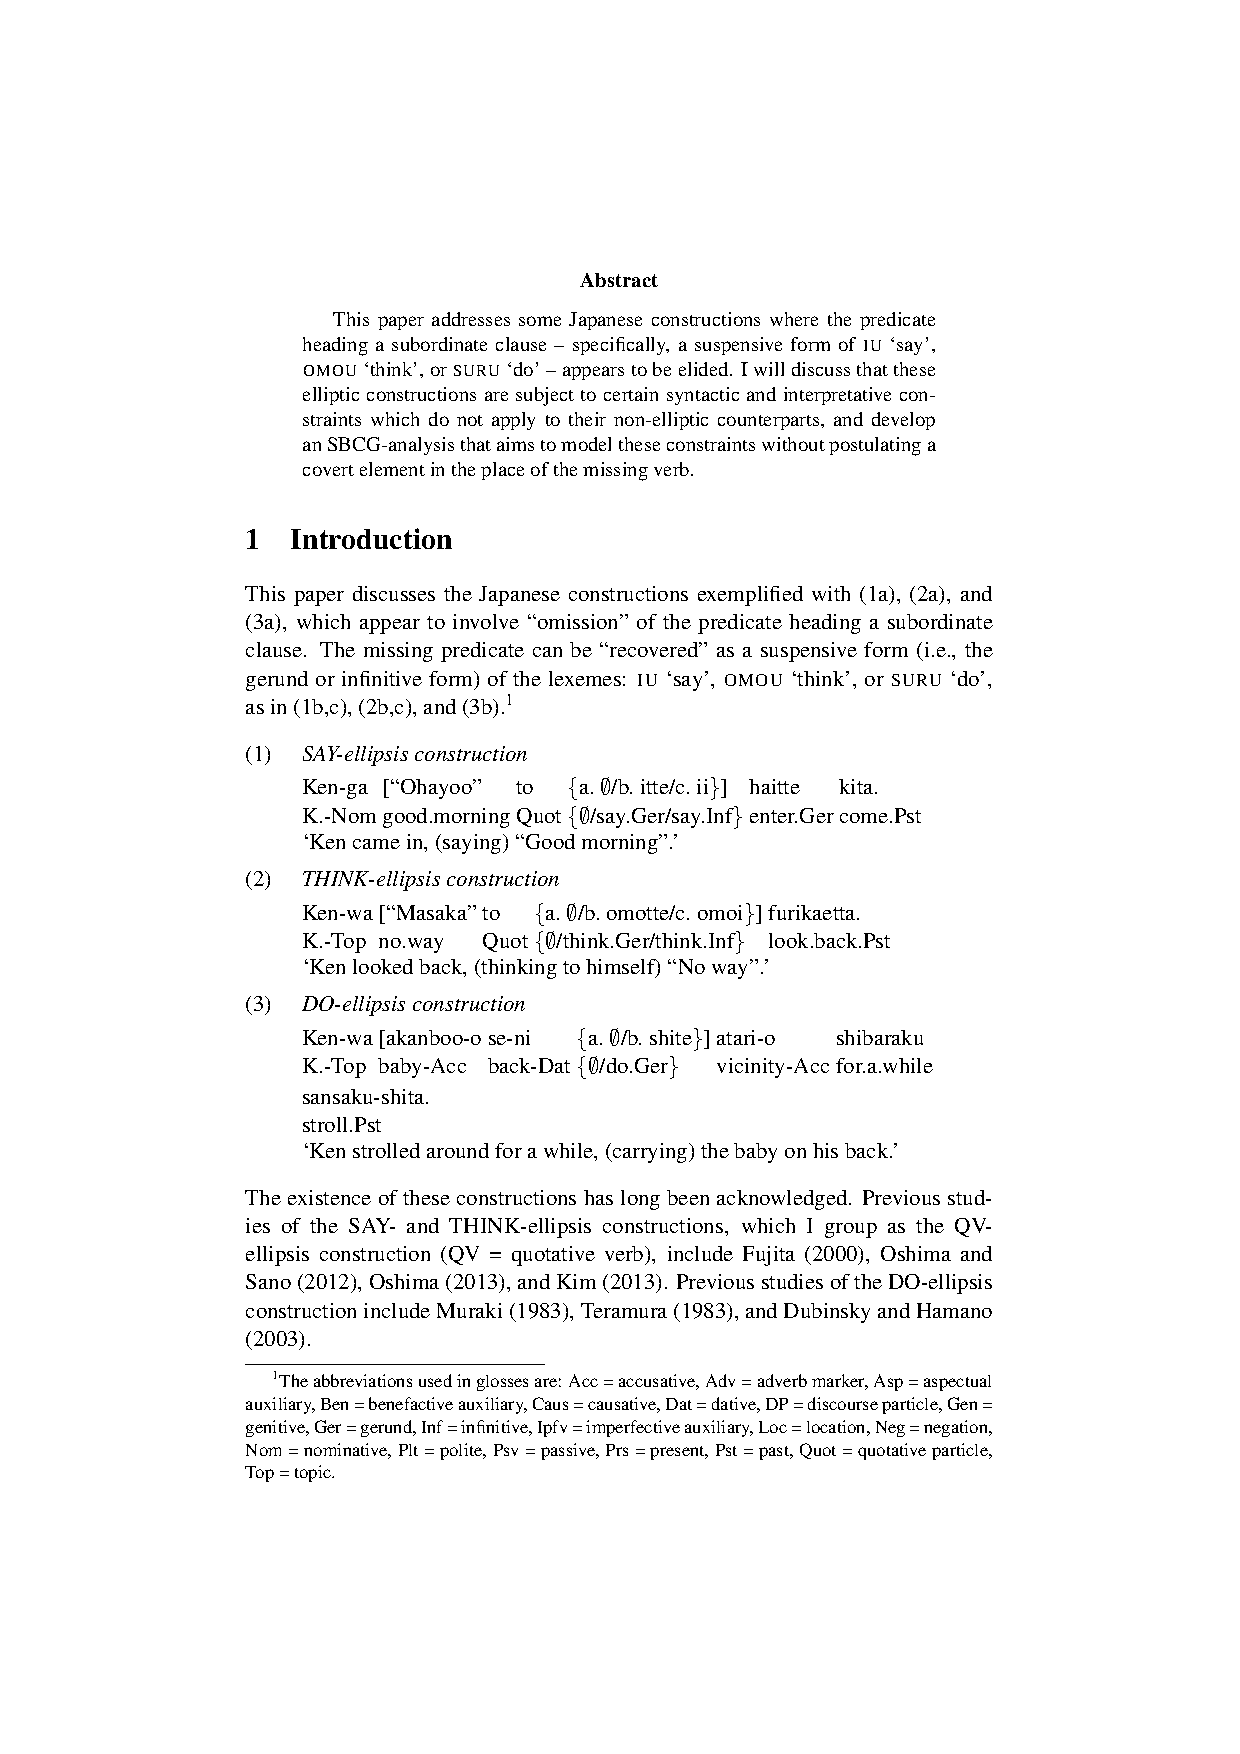
\includepdf[pages=-,pagecommand=\thispagestyle{plain}]{Includes/oshima.pdf}
        \setcounter{page}{177}
        \phantomsection
        \addcontentsline{toc}{section}{Joanna Ut-Seong Sio, Sanghoun Song: Divergence in Expressing Definiteness between {Mandarin} and {Cantonese}}
\thispagestyle{empty}

\begin{center}
  {\huge\bfseries Divergence in Expressing Definiteness between {Mandarin} and {Cantonese}\par}

  \bigskip

~\\
\begingroup
\setlength{\leftskip}{0pt plus 1fill}
\setlength{\rightskip}{0pt plus 1fill}
\setlength{\parindent}{0pt}
\setlength{\parfillskip}{0pt}
  \formatauthor{Joanna Ut-Seong Sio}{\begin{tabular}{@{}c@{}}Nanyang Technological University\end{tabular}}
\formatauthor{Sanghoun Song}{\begin{tabular}{@{}c@{}}Incheon National University\end{tabular}}

\par\endgroup

  \vspace*{8ex}

  Proceedings of the 22nd International Conference on\par Head-Driven Phrase Structure Grammar

  \bigskip

  Nanyang Technological University (NTU), Singapore

  \medskip

  Stefan Müller (Editor)

  \medskip

  2015

  \medskip

  CSLI Publications

  \medskip

  pages 177--194

  \medskip

  \url{http://csli-publications.stanford.edu/HPSG/2015}
\end{center}
\vfill

\noindent



\vfill
\noindent
% APA Style
Sio, Joanna Ut-Seong, \& Song, Sanghoun. 2015. Divergence in Expressing Definiteness between {Mandarin} and {Cantonese}. In Müller, Stefan (Ed.), \emph{{Proceedings of the 22nd International Conference on Head-Driven Phrase Structure Grammar, Nanyang Technological University (NTU), Singapore}}, 177--194. Stanford,
CA: CSLI Publications. \hfill\href{http://creativecommons.org/licenses/by/4.0/}{\includegraphics[height=.75em]{Includes/ccby.eps}}

\newpage
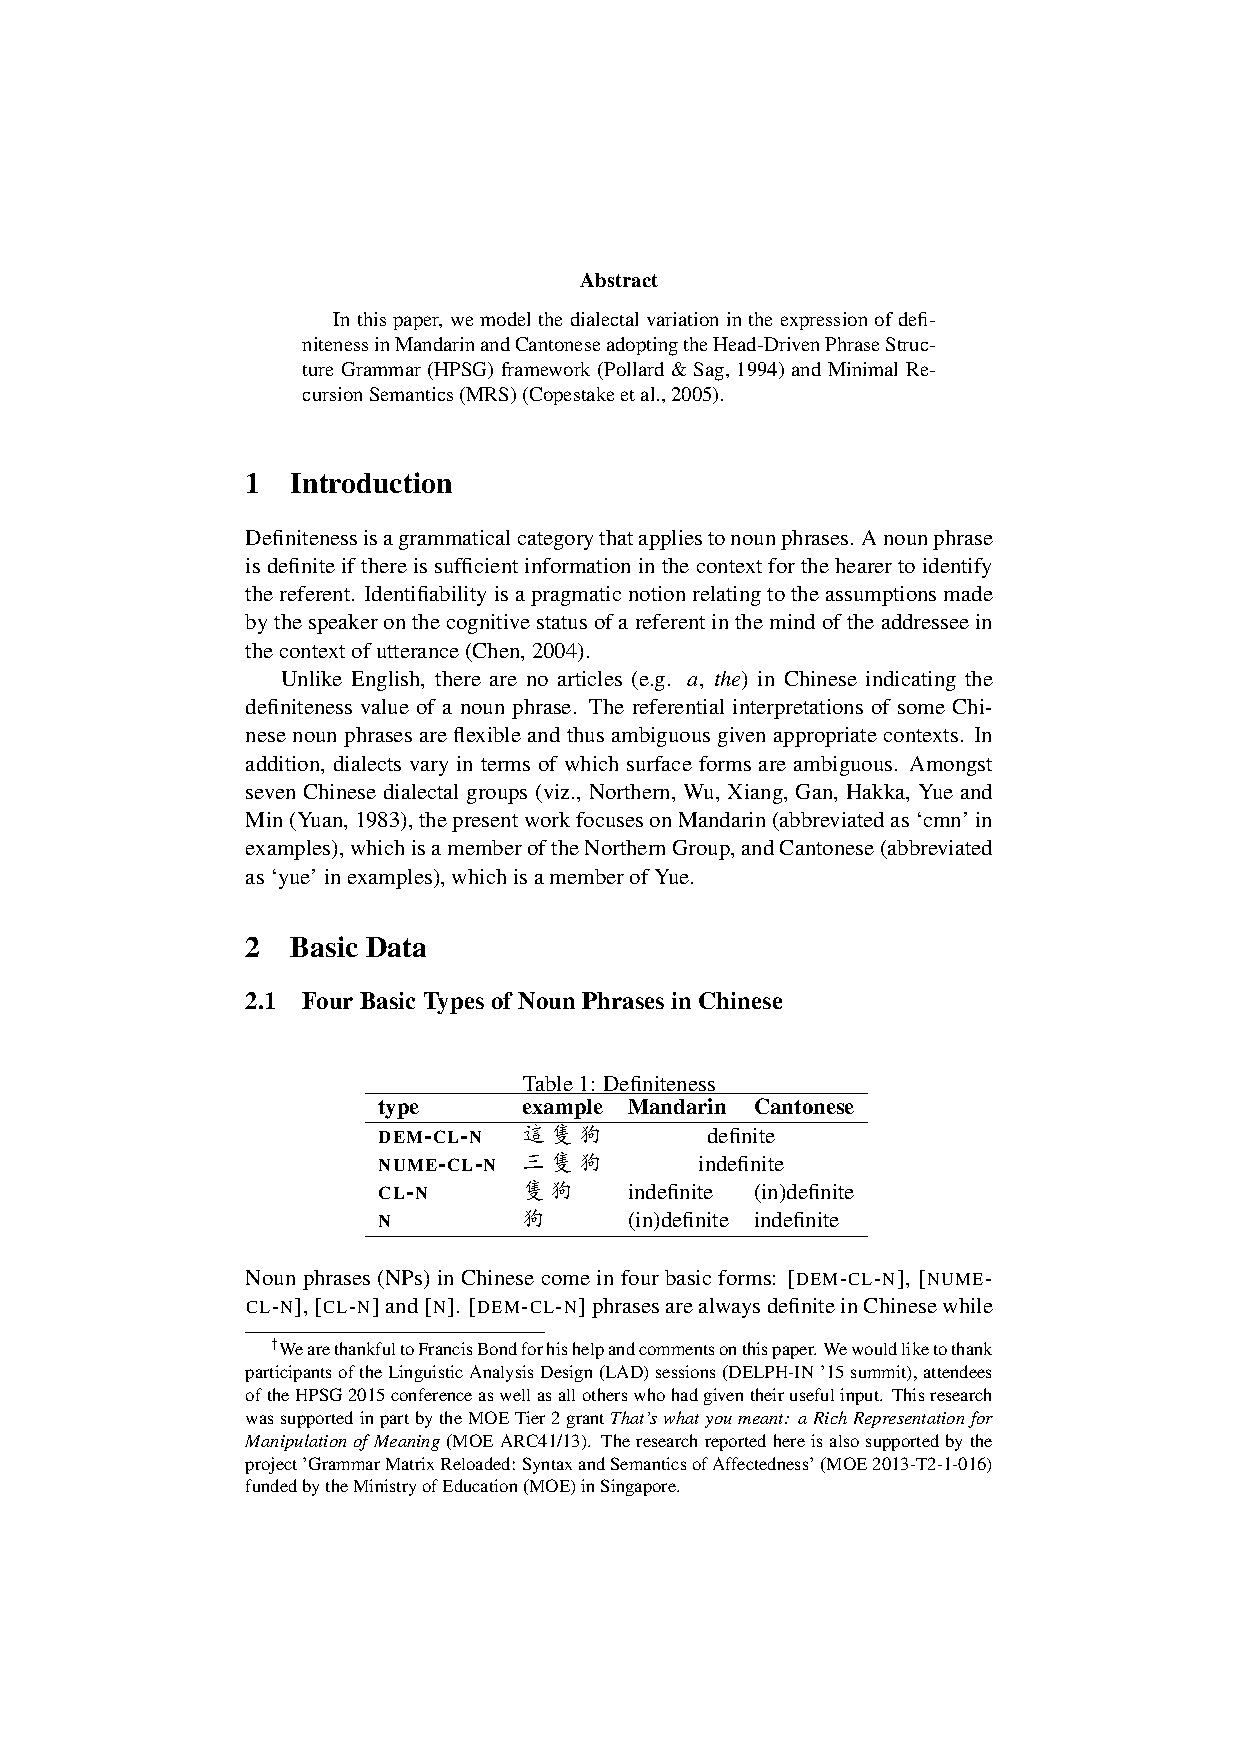
\includepdf[pages=-,pagecommand=\thispagestyle{plain}]{Includes/sio-song.pdf}
        \setcounter{page}{195}
        \phantomsection
        \addcontentsline{toc}{section}{Wenjie Wang, Sanghoun Song, Francis Bond: A Constraint-based Analysis of A-NOT-A Questions in Mandarin Chinese}
\thispagestyle{empty}

\begin{center}
  {\huge\bfseries A Constraint-based Analysis of A-NOT-A Questions in Mandarin Chinese\par}

  \bigskip

~\\
\begingroup
\setlength{\leftskip}{0pt plus 1fill}
\setlength{\rightskip}{0pt plus 1fill}
\setlength{\parindent}{0pt}
\setlength{\parfillskip}{0pt}
  \formatauthor{Wenjie Wang}{\begin{tabular}{@{}c@{}}Nanyang Technological University\end{tabular}}
\formatauthor{Sanghoun Song}{\begin{tabular}{@{}c@{}}Incheon National University\end{tabular}}
\formatauthor{Francis Bond}{\begin{tabular}{@{}c@{}}Nanyang Technological University\end{tabular}}

\par\endgroup

  \vspace*{8ex}

  Proceedings of the 22nd International Conference on\par Head-Driven Phrase Structure Grammar

  \bigskip

  Nanyang Technological University (NTU), Singapore

  \medskip

  Stefan Müller (Editor)

  \medskip

  2015

  \medskip

  CSLI Publications

  \medskip

  pages 195--214

  \medskip

  \url{http://csli-publications.stanford.edu/HPSG/2015}
\end{center}
\vfill

\noindent



\vfill
\noindent
% APA Style
Wang, Wenjie, Song, Sanghoun, \& Bond, Francis. 2015. A Constraint-based Analysis of A-NOT-A Questions in Mandarin Chinese. In Müller, Stefan (Ed.), \emph{{Proceedings of the 22nd International Conference on Head-Driven Phrase Structure Grammar, Nanyang Technological University (NTU), Singapore}}, 195--214. Stanford,
CA: CSLI Publications. \hfill\href{http://creativecommons.org/licenses/by/4.0/}{\includegraphics[height=.75em]{Includes/ccby.eps}}

\newpage
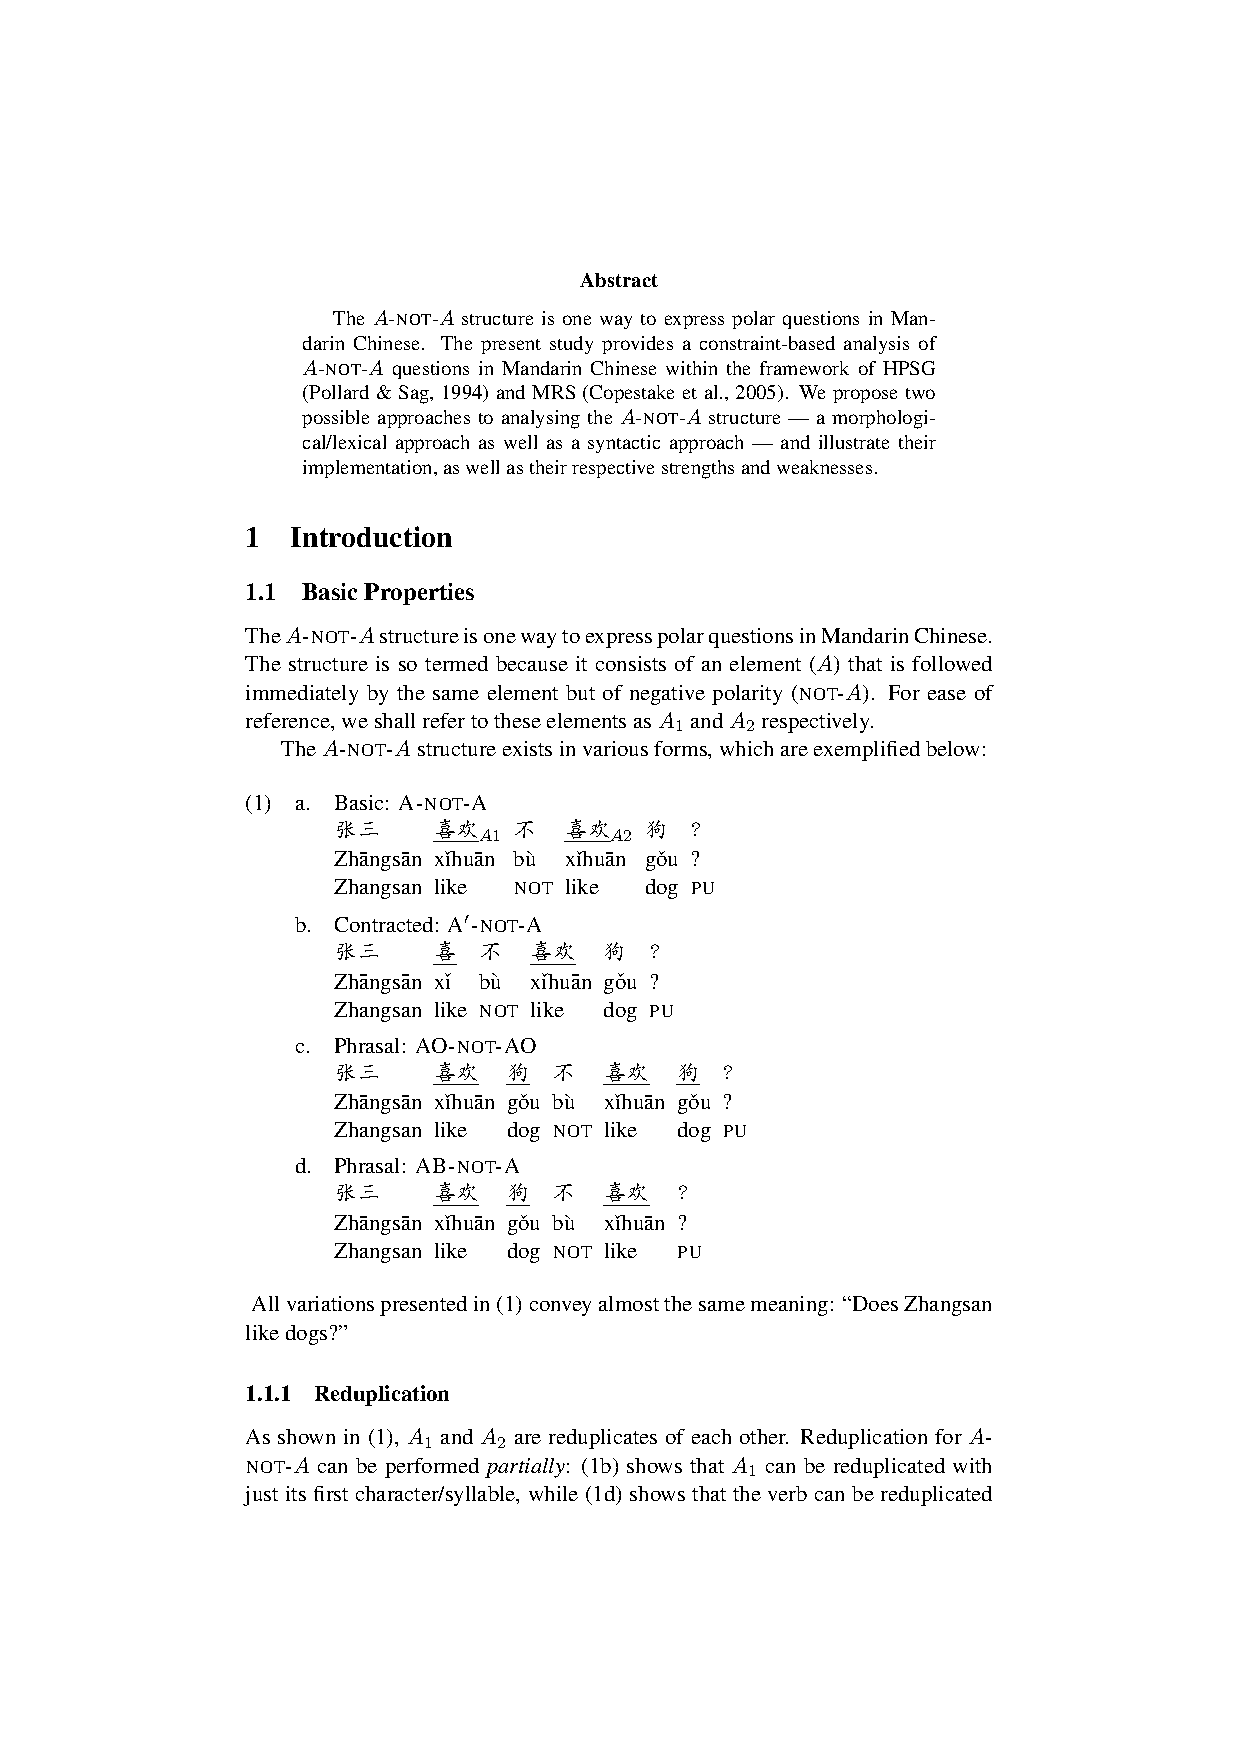
\includepdf[pages=-,pagecommand=\thispagestyle{plain}]{Includes/wsb.pdf}
\part{Contributions to the Workshop}
\thispagestyle{empty}
\newpage
        \setcounter{page}{216}
        \phantomsection
        \addcontentsline{toc}{section}{František Kratochvíl, Benidiktus Delpada: Degrees of affectedness and verbal prefixation in Abui (Papuan)}
\thispagestyle{empty}

\begin{center}
  {\huge\bfseries Degrees of affectedness and verbal prefixation in Abui (Papuan)\par}

  \bigskip

~\\
\begingroup
\setlength{\leftskip}{0pt plus 1fill}
\setlength{\rightskip}{0pt plus 1fill}
\setlength{\parindent}{0pt}
\setlength{\parfillskip}{0pt}
  \formatauthor{František Kratochvíl}{\begin{tabular}{@{}c@{}}Nanyang Technological University, Singapore\end{tabular}}
\formatauthor{Benidiktus Delpada}{\begin{tabular}{@{}c@{}}Nanyang Technological University, Singapore\end{tabular}}

\par\endgroup

  \vspace*{8ex}

  Proceedings of the 22nd International Conference on\par Head-Driven Phrase Structure Grammar

  \bigskip

  Nanyang Technological University (NTU), Singapore

  \medskip

  Stefan Müller (Editor)

  \medskip

  2015

  \medskip

  CSLI Publications

  \medskip

  pages 216--233

  \medskip

  \url{http://csli-publications.stanford.edu/HPSG/2015}
\end{center}
\vfill

\noindent



\vfill
\noindent
% APA Style
Kratochvíl, František, \& Delpada, Benidiktus. 2015. Degrees of affectedness and verbal prefixation in Abui (Papuan). In Müller, Stefan (Ed.), \emph{{Proceedings of the 22nd International Conference on Head-Driven Phrase Structure Grammar, Nanyang Technological University (NTU), Singapore}}, 216--233. Stanford,
CA: CSLI Publications. \hfill\href{http://creativecommons.org/licenses/by/4.0/}{\includegraphics[height=.75em]{Includes/ccby.eps}}

\newpage
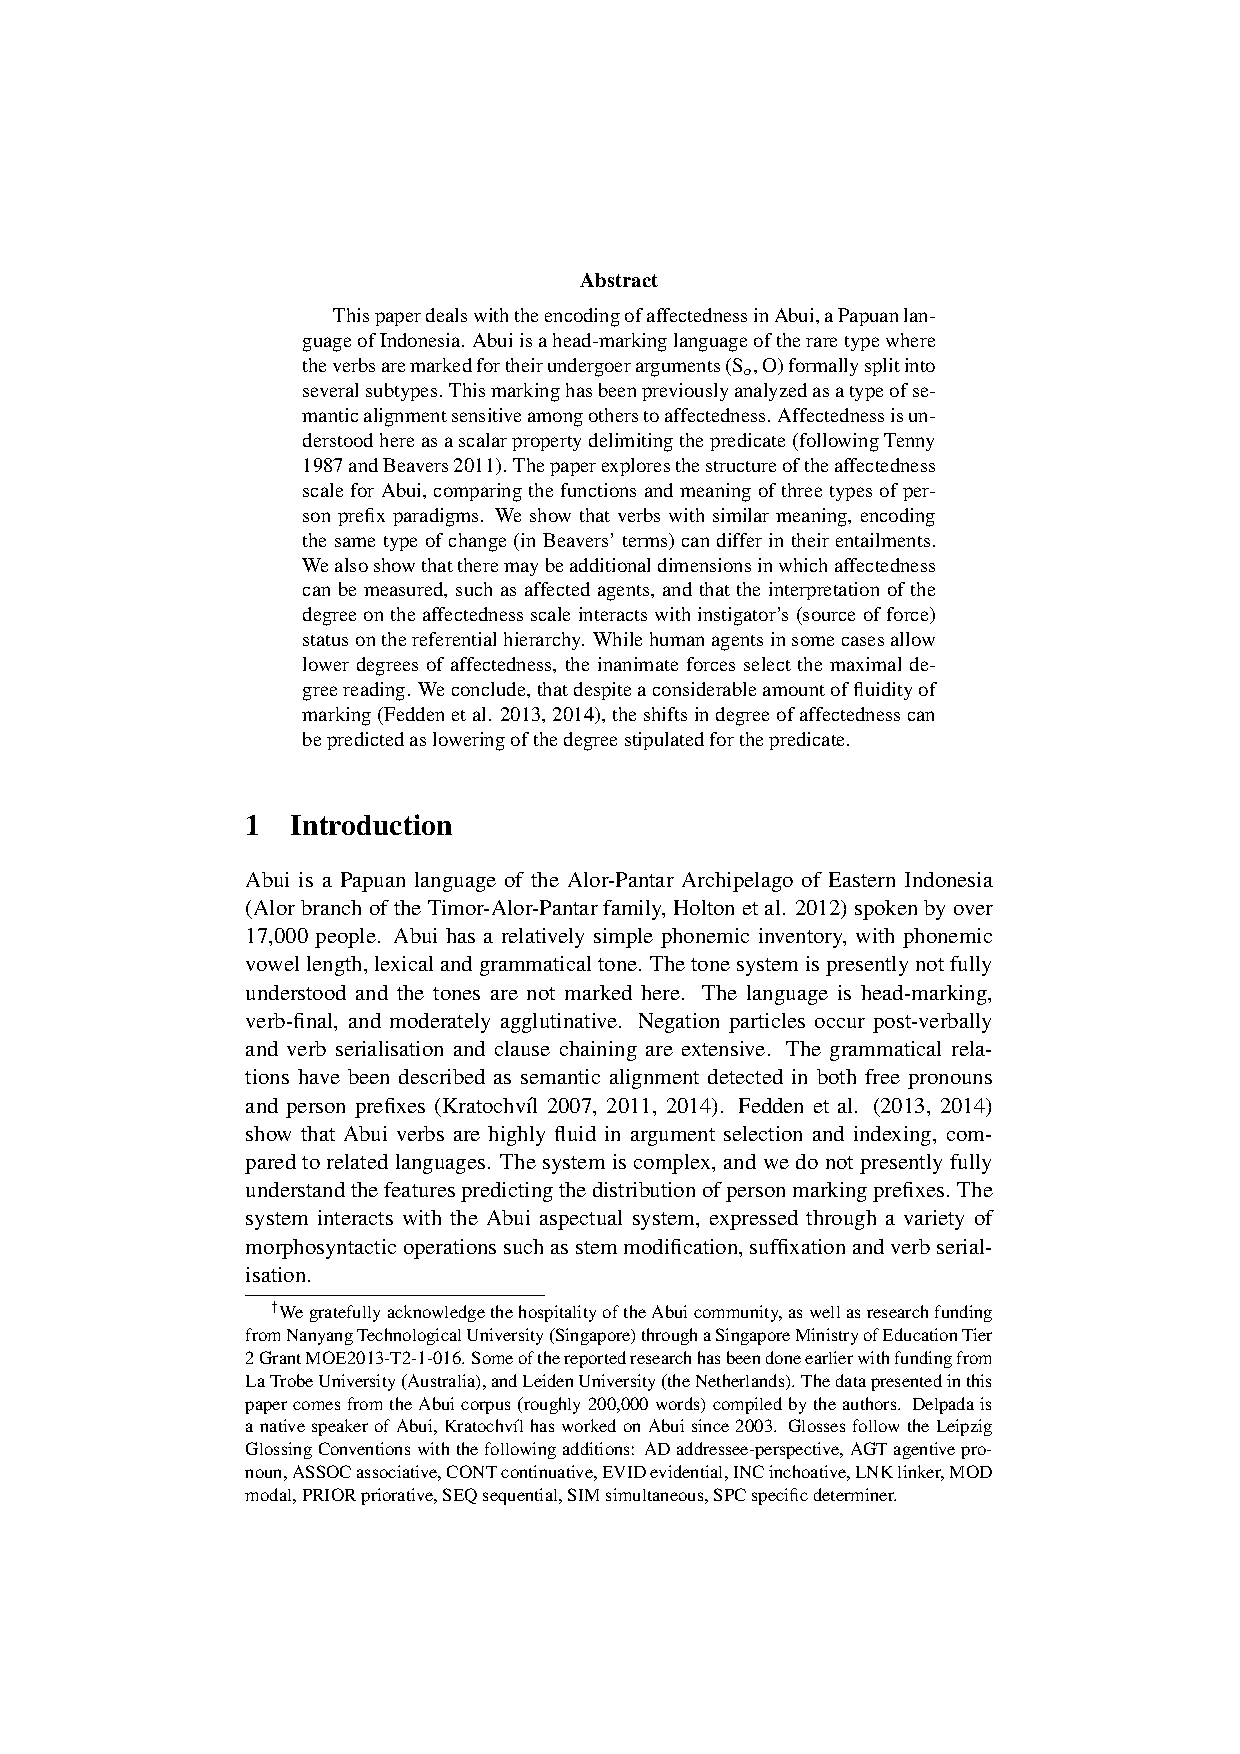
\includepdf[pages=-,pagecommand=\thispagestyle{plain}]{Includes/kratochvil-delpada.pdf}
        \setcounter{page}{234}
        \phantomsection
        \addcontentsline{toc}{section}{Joanna Ut-Seong Sio: Scalarity and the Cantonese post-verbal
particle \emph{can1}}
\thispagestyle{empty}

\begin{center}
  {\huge\bfseries Scalarity and the Cantonese post-verbal
particle \emph{can1}\par}

  \bigskip

~\\
\begingroup
\setlength{\leftskip}{0pt plus 1fill}
\setlength{\rightskip}{0pt plus 1fill}
\setlength{\parindent}{0pt}
\setlength{\parfillskip}{0pt}
  \formatauthor{Joanna Ut-Seong Sio}{\begin{tabular}{@{}c@{}}Nanyang Technological University\end{tabular}}

\par\endgroup

  \vspace*{8ex}

  Proceedings of the 22nd International Conference on\par Head-Driven Phrase Structure Grammar

  \bigskip

  Nanyang Technological University (NTU), Singapore

  \medskip

  Stefan Müller (Editor)

  \medskip

  2015

  \medskip

  CSLI Publications

  \medskip

  pages 234--241

  \medskip

  \url{http://csli-publications.stanford.edu/HPSG/2015}
\end{center}
\vfill

\noindent



\vfill
\noindent
% APA Style
Sio, Joanna Ut-Seong. 2015. Scalarity and the Cantonese post-verbal
particle \emph{can1}. In Müller, Stefan (Ed.), \emph{{Proceedings of the 22nd International Conference on Head-Driven Phrase Structure Grammar, Nanyang Technological University (NTU), Singapore}}, 234--241. Stanford,
CA: CSLI Publications. \hfill\href{http://creativecommons.org/licenses/by/4.0/}{\includegraphics[height=.75em]{Includes/ccby.eps}}

\newpage
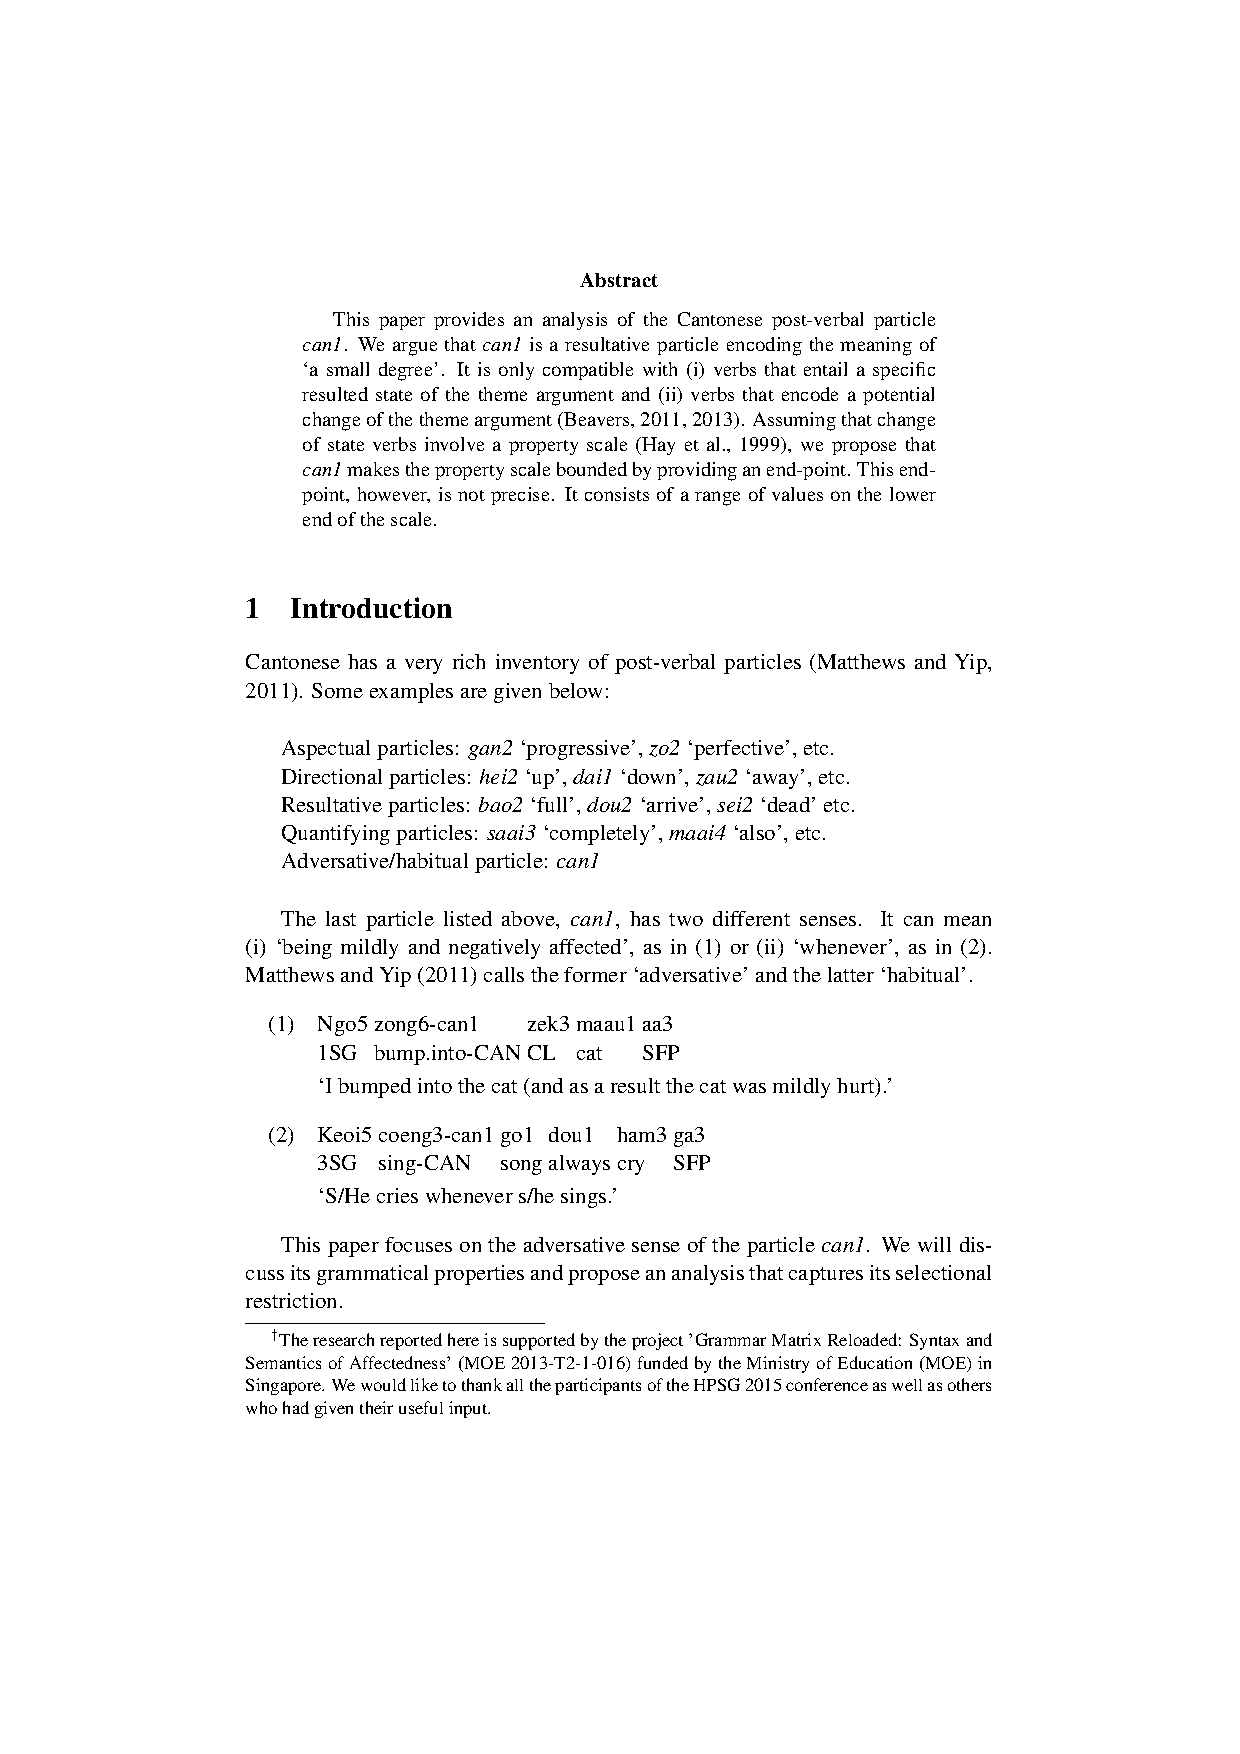
\includepdf[pages=-,pagecommand=\thispagestyle{plain}]{Includes/sio.pdf}
\end{document}
